\documentclass[handout]{beamer}

% \usepackage{beamerthemesplit} // Activate for custom appearance

   \usepackage{mathtools}
   \usepackage{booktabs}
   \usepackage{caption}
    \usepackage{adjustbox} % Used to constrain images to a maximum size    
    \usepackage{array}
    \usepackage{textcomp} % defines textquotesingle
    \usepackage{tikz}
    \usepackage{tikzsymbols}
    \usepackage{adjustbox}
   \usepackage{float}


    \definecolor{lawngreen}{rgb}{0.49, 0.99, 0.0}
    \definecolor{gold}{rgb}{1.0, 0.84, 0.0}
    \definecolor{deepskyblue}{rgb}{0.0, 0.75, 1.0}
    \definecolor{lightgrey}{rgb}{0.83, 0.83, 0.83}


\usetheme{JuanLesPins}
\usecolortheme{dolphin}


\title{Goodreads Topics and Recommendations}
\author{Eitan Angel}    
\date{\today}


%
%\usebackgroundtemplate{%
%\tikz[overlay,remember picture] \node[opacity=0.33, at=(current page.center)] {
%   \adjincludegraphics[height=\paperheight, width=\paperwidth, trim={333 60 0 64},clip]{../instacart-prediction-explorer/output_36_0.png}};
%%   \includegraphics[height=\paperheight,width=\paperwidth]{../instacart-prediction-explorer/output_36_0.png}};
%}

\begin{document}

    	
	\newcolumntype{H}{>{\setbox0=\hbox\bgroup}c<{\egroup}@{}}
	\newcolumntype{Z}{>{\setbox0=\hbox\bgroup}c<{\egroup}@{\hspace*{-\tabcolsep}}}

\frame{

\titlepage}



\frame{\tableofcontents[hideallsubsections]}

\usebackgroundtemplate{%
}
\section{Introduction}
\subsection{Problem: Goodreads Topics, Profiles, and Recommendations}\label{problem}

\begin{frame}
\href{https://www.goodreads.com}{Goodreads} is a social site for readers. Readers rate, tag, and discuss books.\vfill
\begin{description}[<+->]
\item[Topics:] `Learn'' book topics from reader ratings data. \vfill
\begin{itemize}[<+->]
\item Topics are interpretable; user-generated tags assist\vfill
\item Simple way to create ``Because you liked Harry Potter\ldots'' product feature.\vfill
\end{itemize}
\item[Profiles:] Topics extracted provide a profile for each reader to aid targeted marketing.\vfill
\item[Recommendations:] Individually-targeted book recommendations for existing users. \vfill
\end{description}
\end{frame}



\subsection{Data: \href{https://github.com/zygmuntz/goodbooks-10k}{Goodbooks-10k}}\label{data}

\begin{frame}

\begin{itemize}[<+->]
\item The most popular 10,000 books on Goodreads by ratings with
\begin{itemize}[<+->]
\item author(s),
\item title(s),
\item language,
\item count of ratings, 
\item number of ratings
\end{itemize}
\vfill
\item Book ratings by over 50,000 users from 1 -- 5.
\vfill
\item User-generated tags: A count for each of the top 100 tags for each of the 10,000 books.
\end{itemize}

\end{frame}


\subsection{Approach: Collaborative Filtering via Matrix Factorization}\label{approach}

\begin{frame}
\begin{block}{Nonnegative Matrix Factorization}
\setlength\abovedisplayskip{0pt}
For user-ratings matrix $V$, make a low-rank approximation
\[ V \approx WH\]
\end{block}
\vfill

\begin{columns}
\column{0.65\linewidth}
\begin{itemize}[<+->]
\item Choose number of latent features
\item $W$ a matrix of user latent features
\item $H$ a matrix of book latent features
\item %Matrix ``completion'' 
$A =WH$ ``fills-in'' blank ratings in $V$
\item Recommend top values of rows of $A$
\item $H$ rows weight tags for topic extraction
\end{itemize}
\column{0.35\linewidth}
\begin{block}{Ratings Matrix $V$}
\centering
\[\left[\begin{array}{|r|cccc|}\hline
\text{Sam} & ? & 4 & ? & 1 \\
\text{Jim} & 2 & 5 & ? & ? \\
\text{Lex} & 5 & ? & ? & 4 \\
\text{Kat} & 4 & 1 & 3 & 5 \\
\text{Bob} & ? & ? & 4 & 5 \\\hline
\end{array}\right]\]
\end{block}
\end{columns}
\end{frame}





\section%[RawData]
{Exploration}\label{exploration}

\subsection{Most Rated Books}\label{most-rated-books}

\begin{frame}


\begin{table}
\begin{tabular}{lHlHHHHHZ}
\toprule
                     authors &  year &                                              title & language\_code &  avg\_rating &  ratings\_count &  ratings &  work\_text\_reviews\_count &  ratings\_ratio \\
\midrule
             Suzanne Collins &                     2008.0 &            The Hunger Games (The \ldots &           eng &            4.34 &        4780653 &             4942365 &                   155254 &       0.031413 \\
 J.K. Rowling, Mary GrandPr\'e &                     1997.0 &  Harry Potter and the Sorcerer's\ldots &           eng &            4.44 &        4602479 &             4800065 &                    75867 &       0.015805 \\
             Stephenie Meyer &                     2005.0 &                            Twilight (Twilight, \#1) &         en-US &            3.57 &        3866839 &             3916824 &                    95009 &       0.024257 \\
                  Harper Lee &                     1960.0 &                              To Kill a Mockingbird &           eng &            4.25 &        3198671 &             3340896 &                    72586 &       0.021727 \\
         F. Scott Fitzgerald &                     1925.0 &                                   The Great Gatsby &           eng &            3.89 &        2683664 &             2773745 &                    51992 &       0.018744 \\
                  John Green &                     2012.0 &                             The Fault in Our Stars &           eng &            4.26 &        2346404 &             2478609 &                   140739 &       0.056781 \\
               Veronica Roth &                     2011.0 &                          Divergent (Divergent, \#1) &           eng &            4.24 &        1903563 &             2216814 &                   101023 &       0.045571 \\
              J.R.R. Tolkien &                     1937.0 &                                         The Hobbit &         en-US &            4.25 &        2071616 &             2196809 &                    37653 &       0.017140 \\
                 Jane Austen &                     1813.0 &                                Pride and Prejudice &           eng &            4.24 &        2035490 &             2191465 &                    49152 &       0.022429 \\
               J.D. Salinger &                     1951.0 &                             The Catcher in the Rye &           eng &            3.79 &        2044241 &             2120637 &                    44920 &       0.021182 \\
\bottomrule
\end{tabular}
    \caption[Most Rated Books]{The most popular books on Goodreads.}
     \label{tbl:most-rated-books}
\end{table}


\end{frame}

\subsection{Most Highly-Rated Books}\label{most-highly-rated-books}

\begin{frame}
 

\begin{table}
\begin{tabular}{lHlHHHHHZ}
\toprule
                                    authors &  original\_publication\_year &                                              title & language\_code &  average\_rating &  ratings\_count &  work\_ratings\_count &  work\_text\_reviews\_count &  ratings\_ratio \\
\midrule
                             Bill Watterson &                     2005.0 &                     The Complete Calvin and Hobbes &           eng &            4.82 &          28900 &               29968 &                      861 &       0.028731 \\
                J.K. Rowling, \ldots &                     2003.0 &  Harry Potter Boxed Set, Books 1-5 \ldots. &           eng &            4.77 &          33220 &               33424 &                      156 &       0.004667 \\
                          Brandon Sanderson &                     2014.0 &     Words of Radiance (The Stormlight \ldots &           eng &            4.77 &          73572 &              108176 &                     7261 &       0.067122 \\
                            Francine Rivers &                     1993.0 &                           Mark of the Lion Trilogy &         en-US &            4.76 &           9081 &                9547 &                      731 &       0.076569 \\
 Anonymous \ldots &                     2002.0 &                                    ESV Study Bible &           eng &            4.76 &           8953 &               10784 &                      262 &       0.024295 \\
                             Bill Watterson &                     1996.0 &  It's a Magical World: A Calvin and \ldots &           eng &            4.75 &          22351 &               23429 &                      264 &       0.011268 \\
                             Bill Watterson &                     1996.0 &  There's Treasure Everywhere: A Calvin \ldots &           eng &            4.74 &          16766 &               17285 &                      149 &       0.008620 \\
                               J.K. Rowling &                     1998.0 &           Harry Potter Boxset (Harry Potter, \#1-7) &           eng &            4.74 &         190050 &              204125 &                     6508 &       0.031882 \\
                               J.K. Rowling &                     2005.0 &       Harry Potter Collection (Harry Potter, \#1-6) &           eng &            4.73 &          24618 &               26274 &                      882 &       0.033569 \\
                             Bill Watterson &                     1992.0 &                The Indispensable Calvin and Hobbes &           eng &            4.73 &          14597 &               16911 &                      325 &       0.019218 \\
\bottomrule
\end{tabular}
    \caption[Most Highly-Rated Books]{Calvin \& Hobbes and Harry Potter dominate the average ratings.}
     \label{tbl:most-highly-rated-books}
\end{table}


\end{frame}




\section{Models}\label{models}


\subsection{Ratings}\label{ratings}


\begin{frame}

\begin{figure}
    \begin{center}
    \adjustimage{max size={0.9\linewidth}{0.9\paperheight}}{../report/exploration_images/output_38_0.png}
    \end{center}
    \caption[Distribution of User Ratings]{Ratings of 4 or 5 are by far most common.}
     \label{fig:average-rating-reviews-count}
\end{figure}
\end{frame}

\begin{frame}
\begin{figure}

    \begin{center}
    \adjustimage{max size={0.9\linewidth}{0.9\paperheight}}{../report/exploration_images/output_48_0.png}
    \end{center}
    \caption[Distribution of Ratings by User]{The range of reviews by user is 19--200.}
     \label{fig:ratings-by-user}
     \end{figure}

\end{frame}

\subsection{Ratings Matrix}\label{ratings-matrix}

\begin{frame}

\begin{figure}
    \centering
    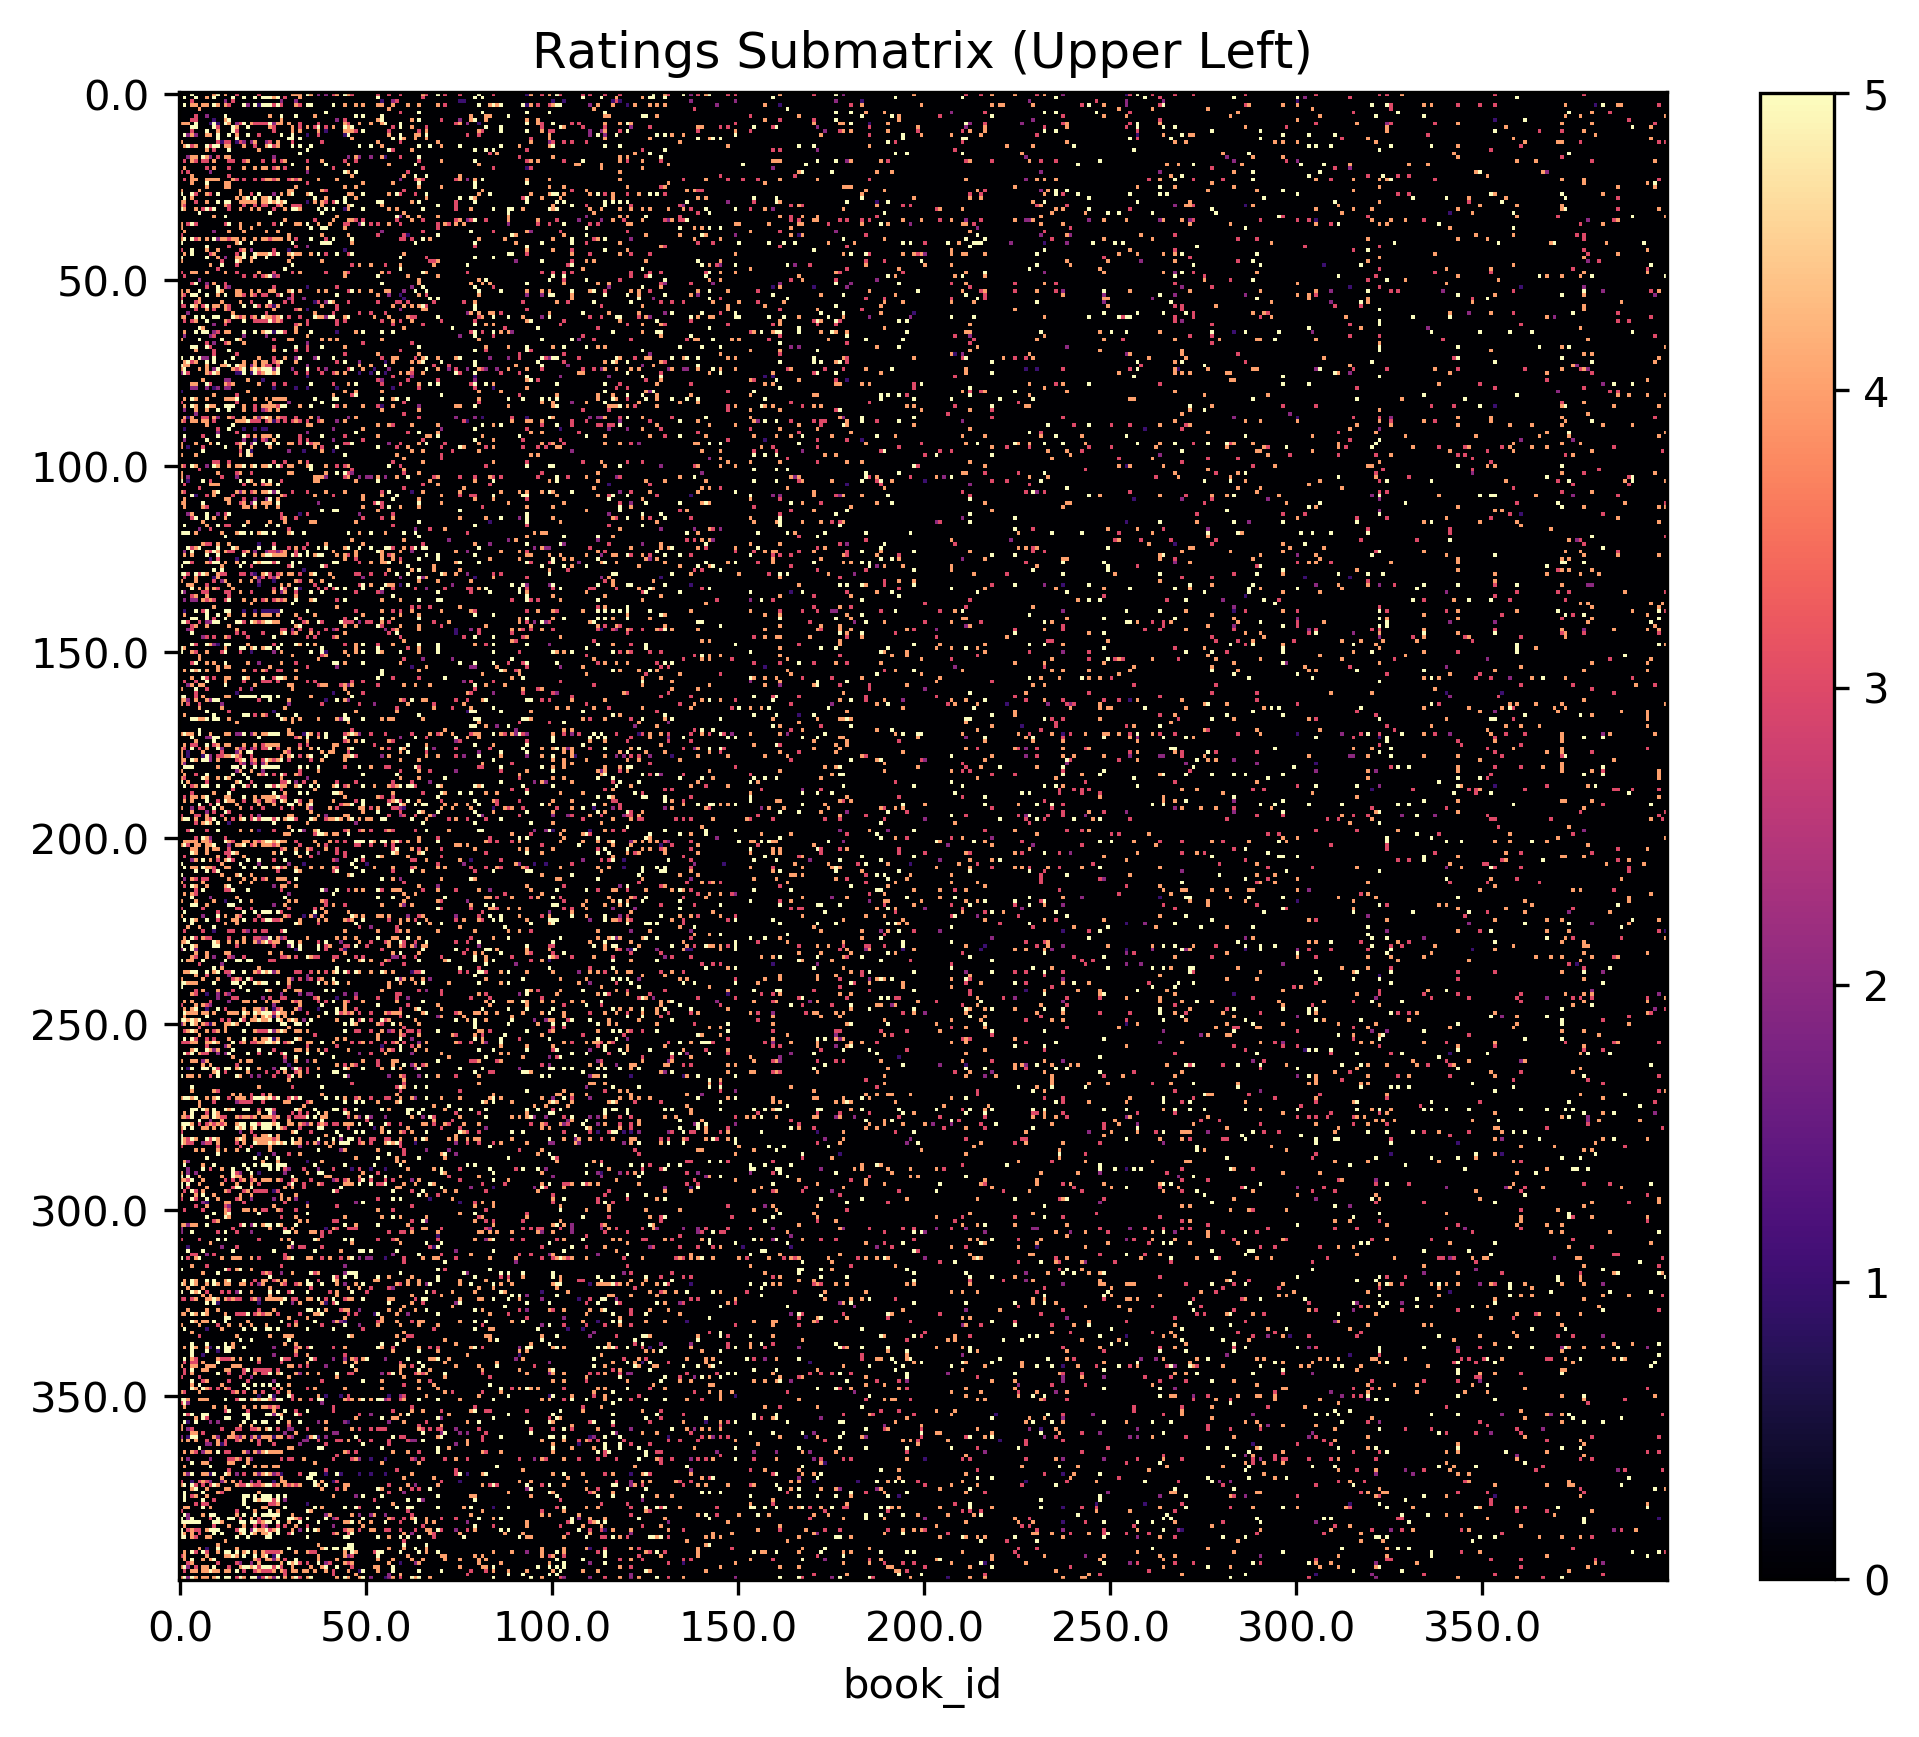
\includegraphics[height=0.7\paperheight, width=0.7\linewidth]{../image/goodreads-models/ratings-submatrix-upper-left.png}
%    \vspace{-30pt}
    \caption[Ratings Submatrix]{The first 400 rows and columns of the ratings matrix.}
     \label{fig:ratings-submatrix-upper-left}
\end{figure}
\end{frame}

\begin{frame}
 

\begin{figure}
    \centering
    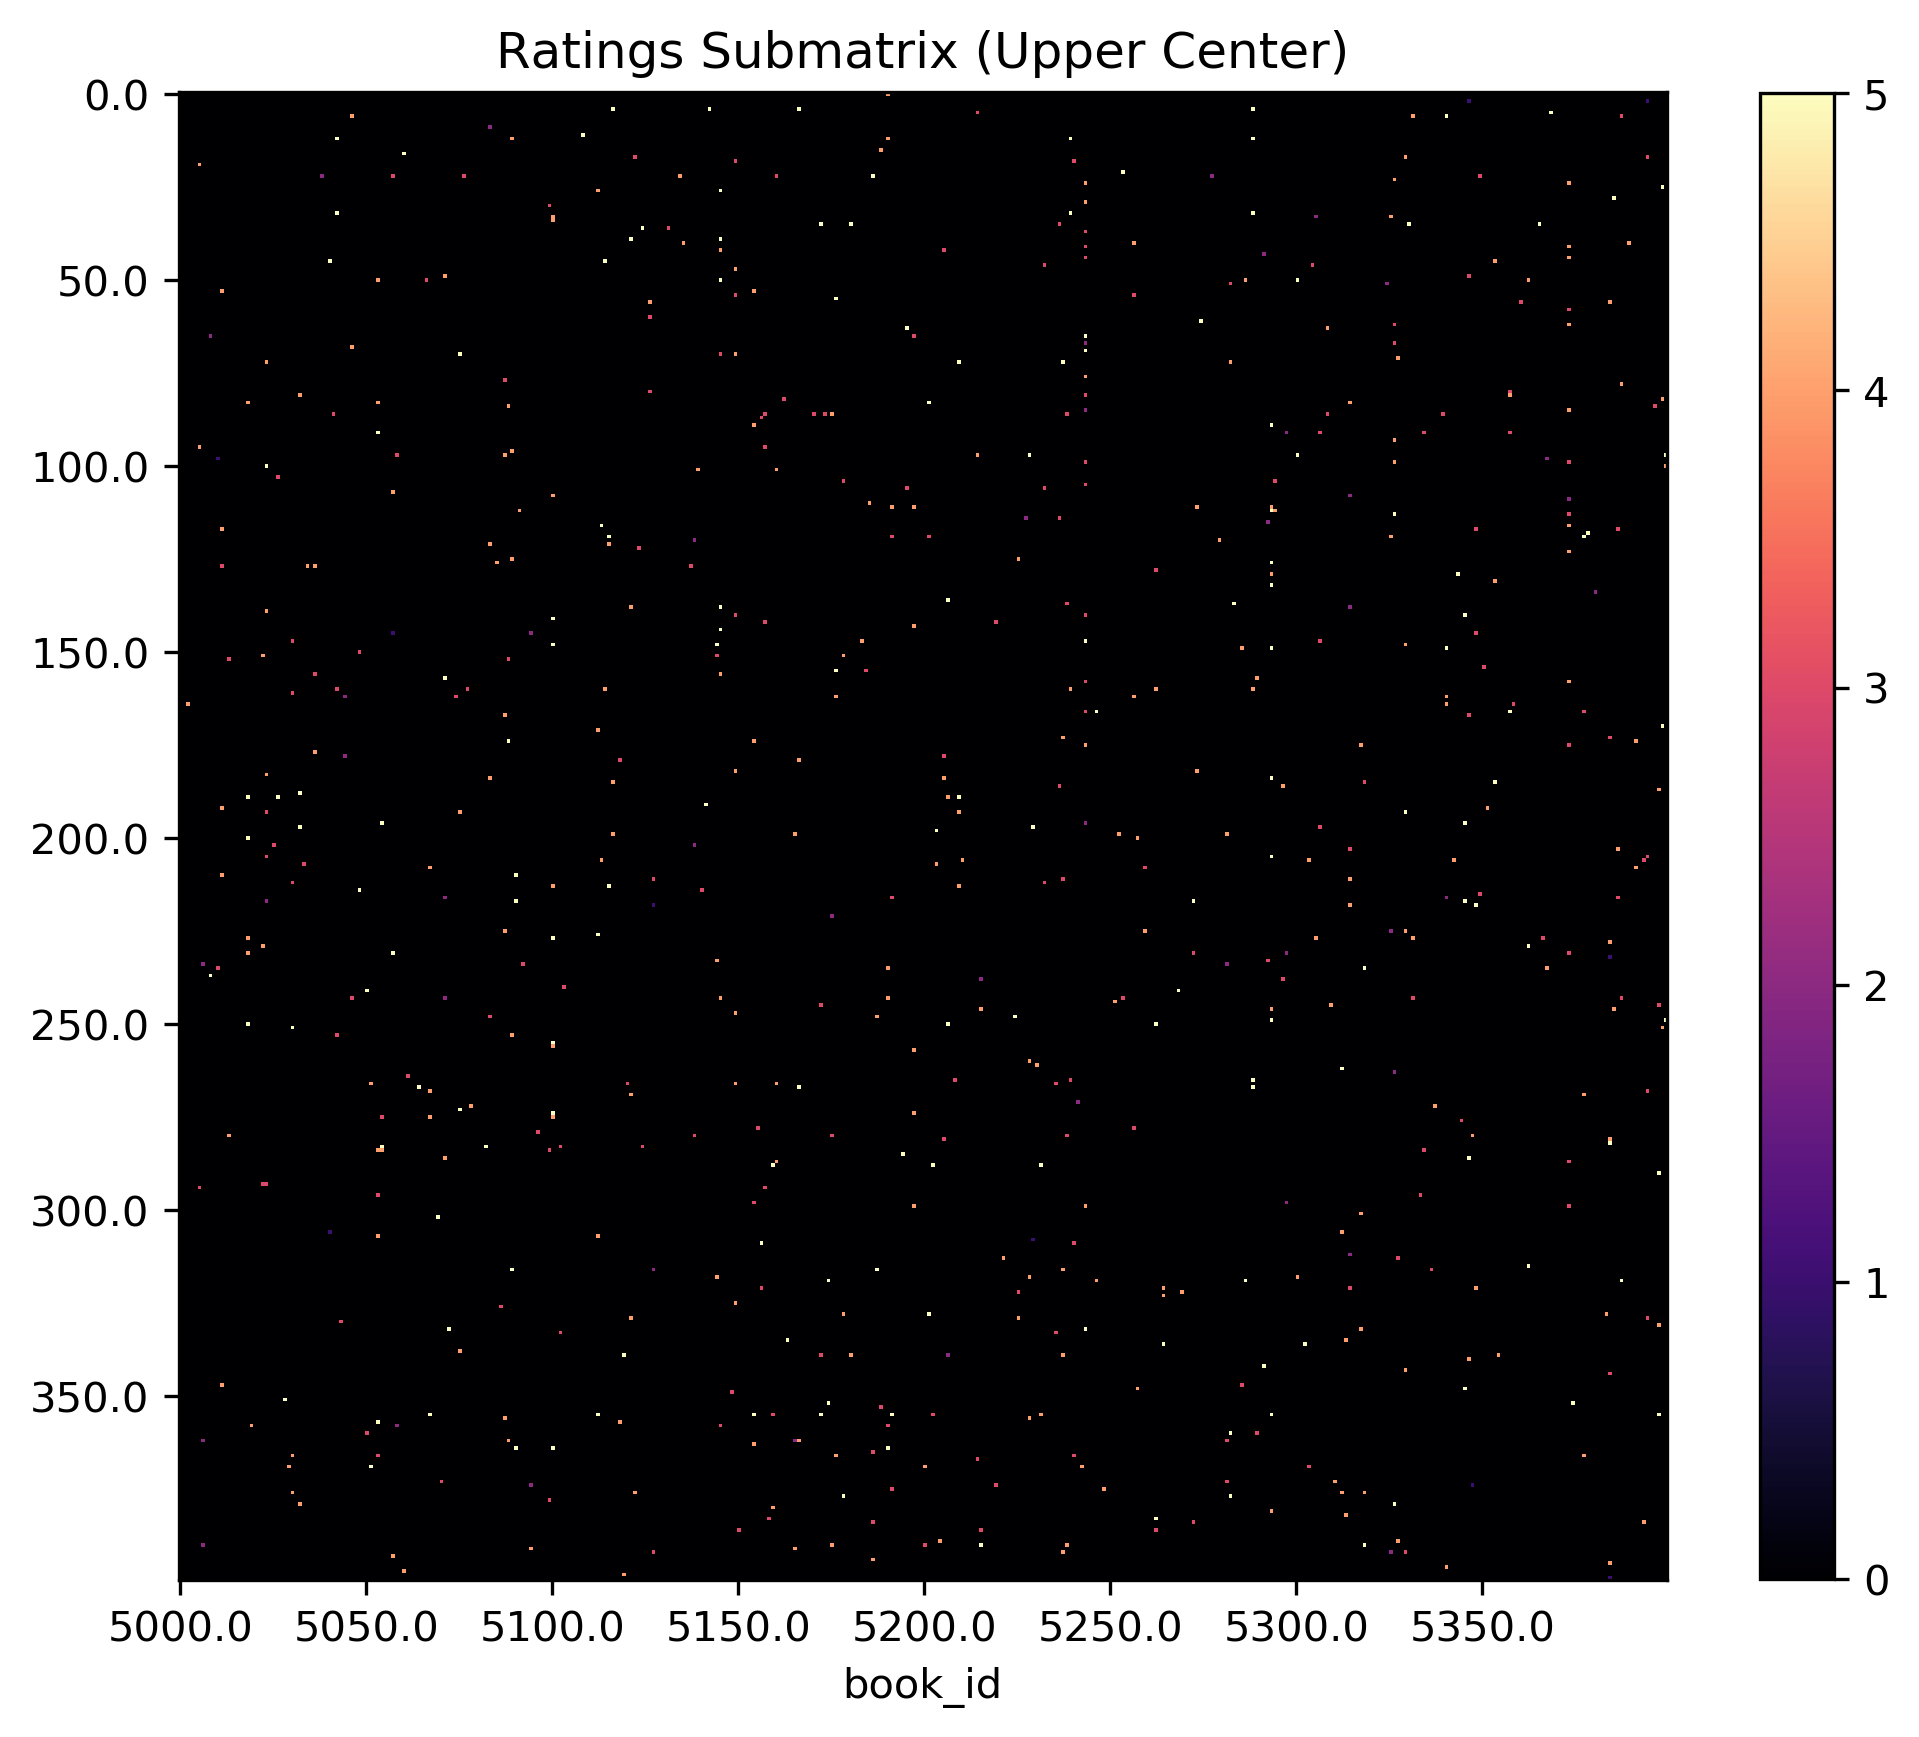
\includegraphics[height=0.7\paperheight, width=0.7\linewidth]{../image/goodreads-models/ratings-submatrix-upper-center.png}
%    \vspace{-30pt}
    \caption[Ratings Submatrix (Center)]{The upper center of the ratings matrix. \texttt{book\_id} is ordered by overall ratings. The density of the matrix is 1.12\%.}
     \label{fig:ratings-submatrix-upper-left-center}
\end{figure}
\end{frame}



\subsection{Baseline}\label{baseline}


\begin{frame}
 \begin{figure}[t]
  %  \centering
    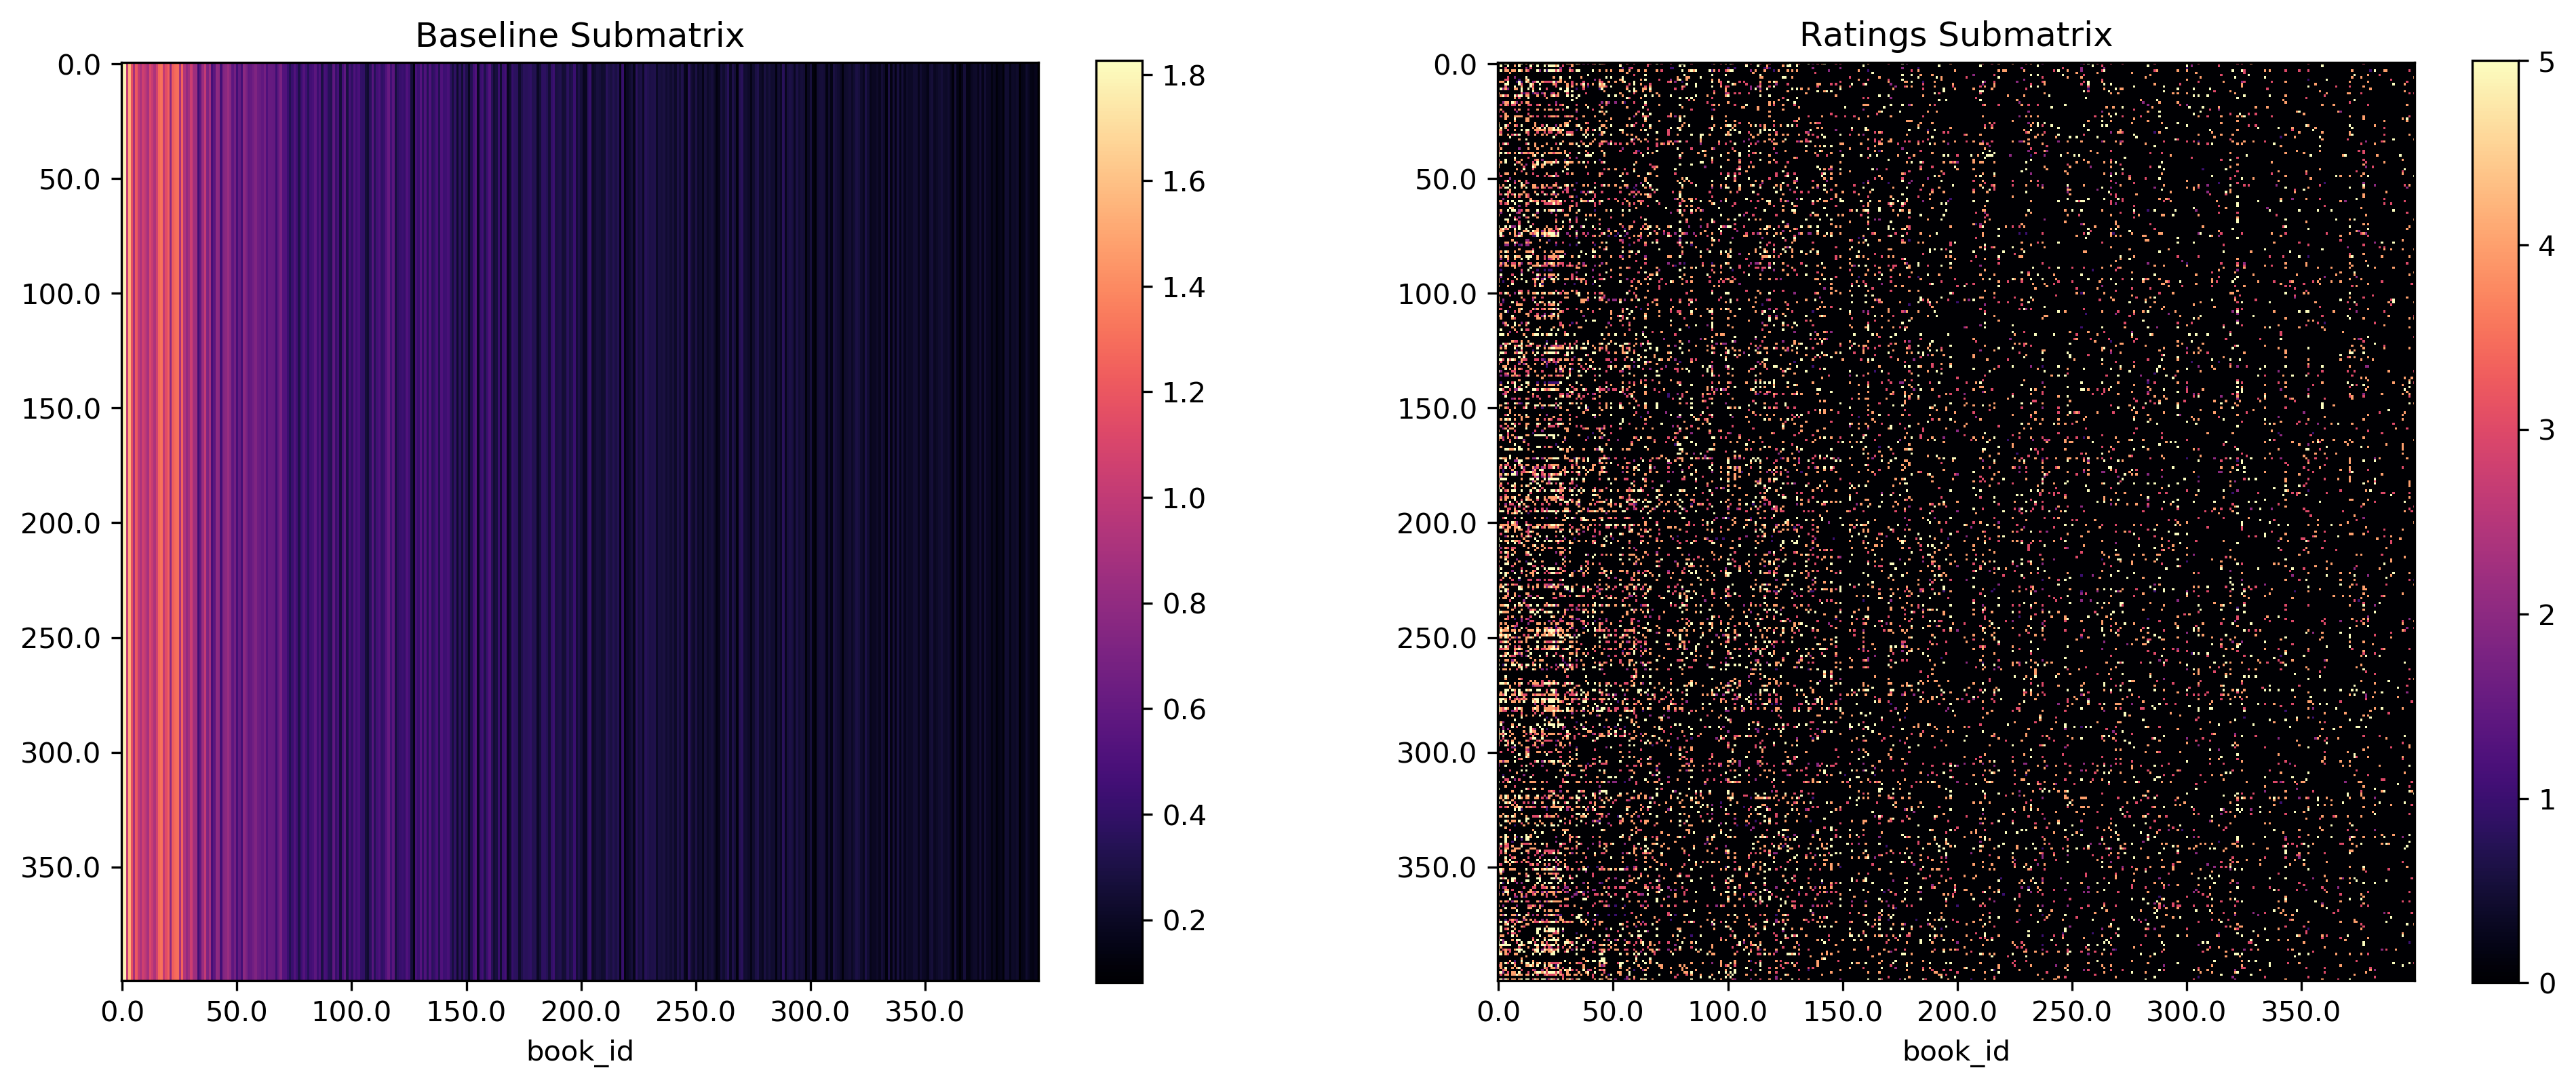
\includegraphics[width=\linewidth]{../image/goodreads-models/baseline-matrix.png}
%    \vspace{-30pt}
    \caption[Baseline matrix]{The mean book rating along each column including no ratings.}
     \label{fig:baseline-matrix}
\end{figure}
\end{frame}

\subsection{$k=1$}\label{k-1}

\begin{frame}
 \begin{figure}[t]
  %  \centering
    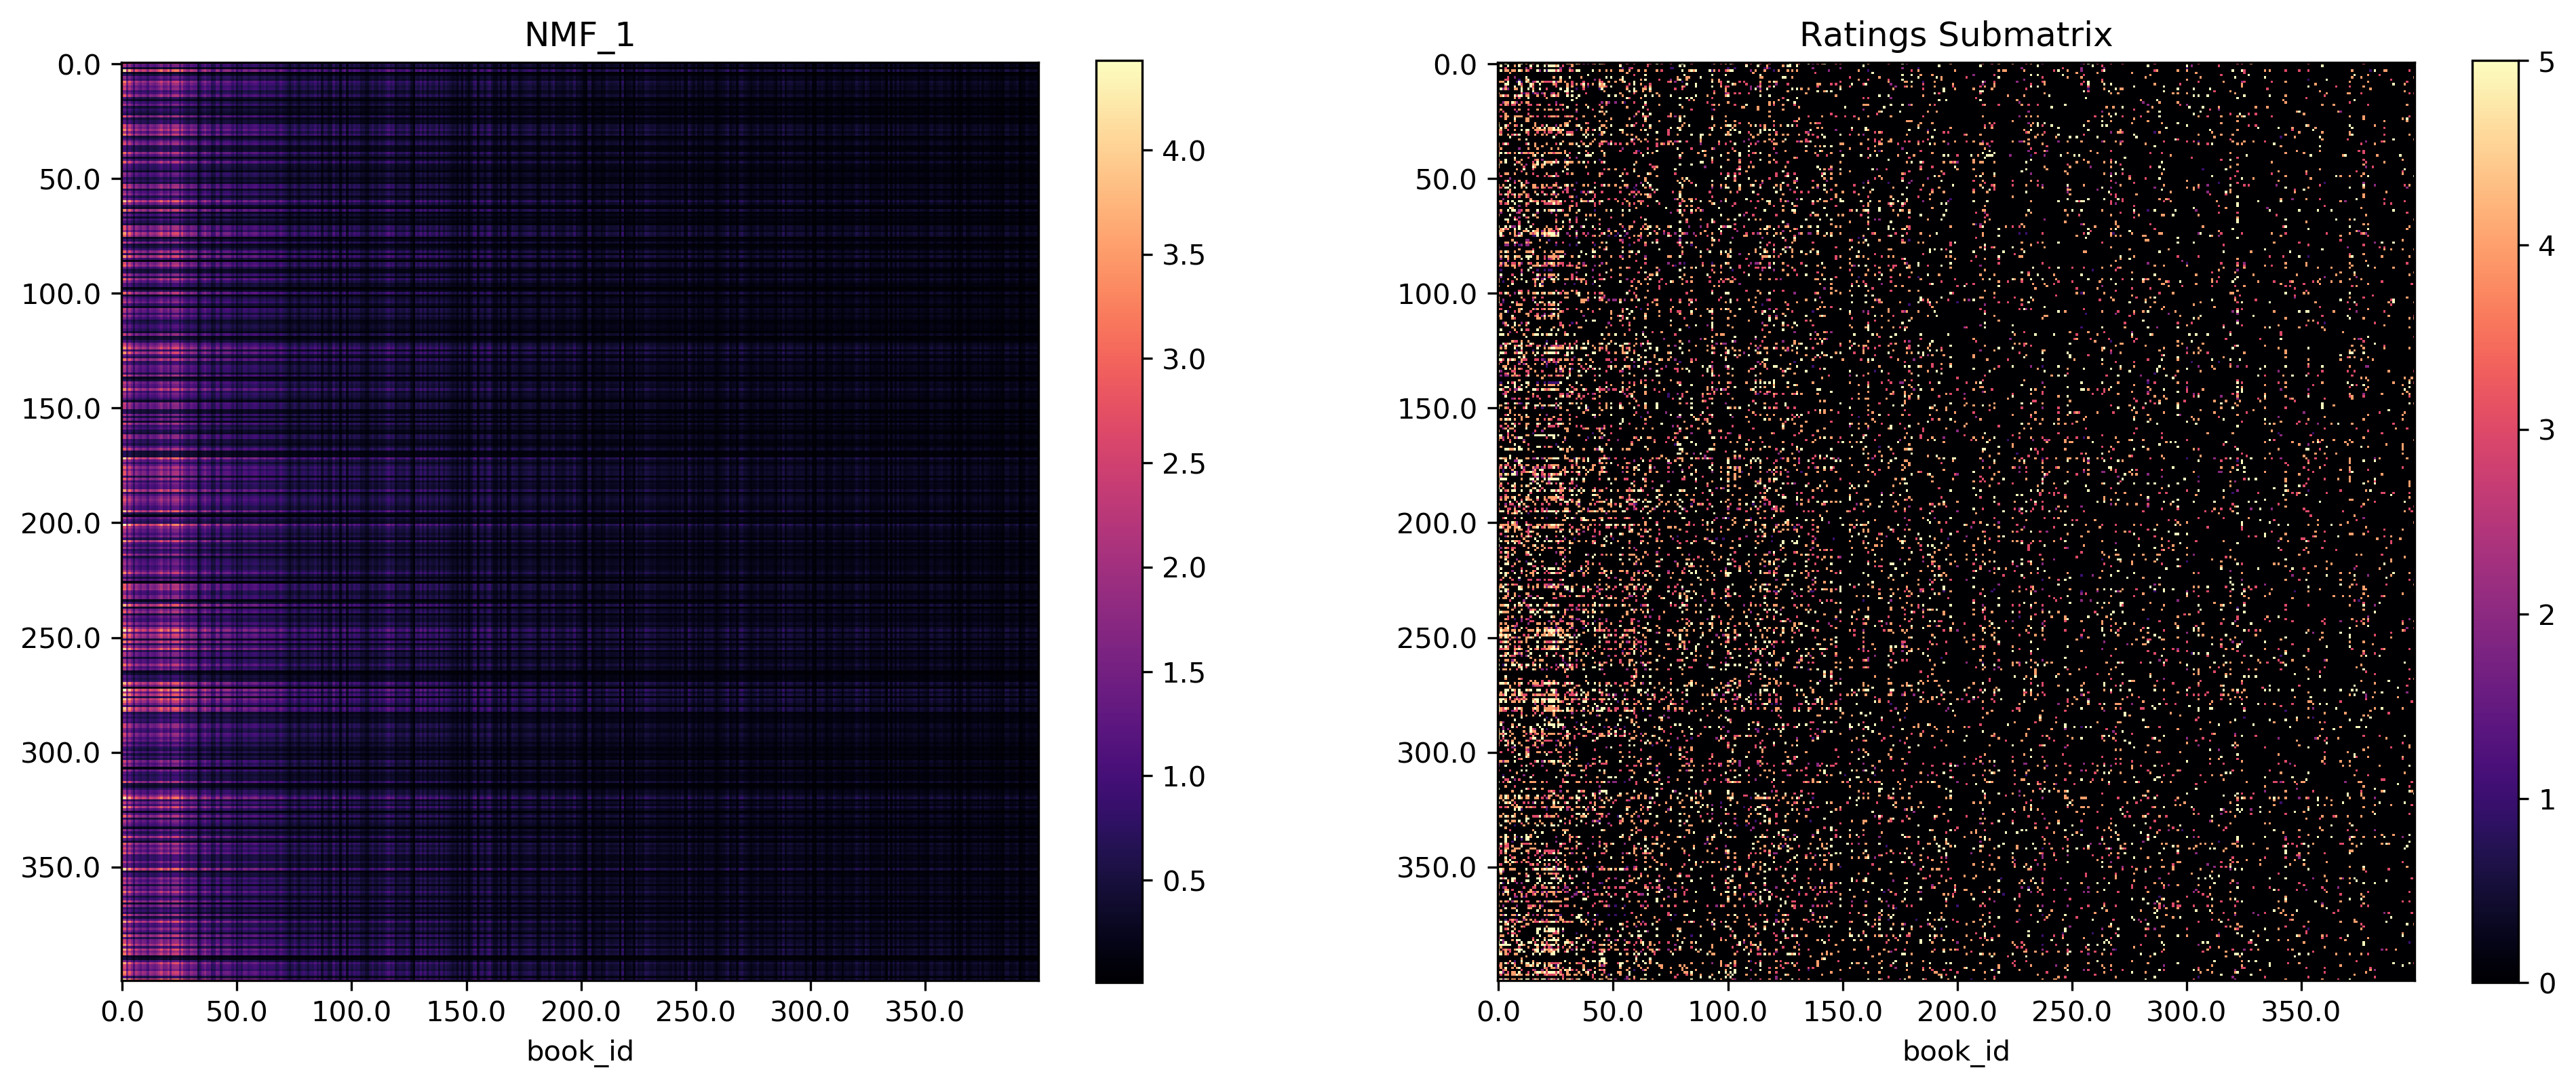
\includegraphics[width=\linewidth]{../image/goodreads-models/nmf-1-left.png}
%    \vspace{-30pt}
    \caption[NMF-1]{The matrix reconstruction ($k=1$).}
     \label{fig:nmf-1}
\end{figure}
\end{frame}

\subsection{$k=10$}\label{k-10}

\begin{frame}
 \begin{figure}[t]
  %  \centering
    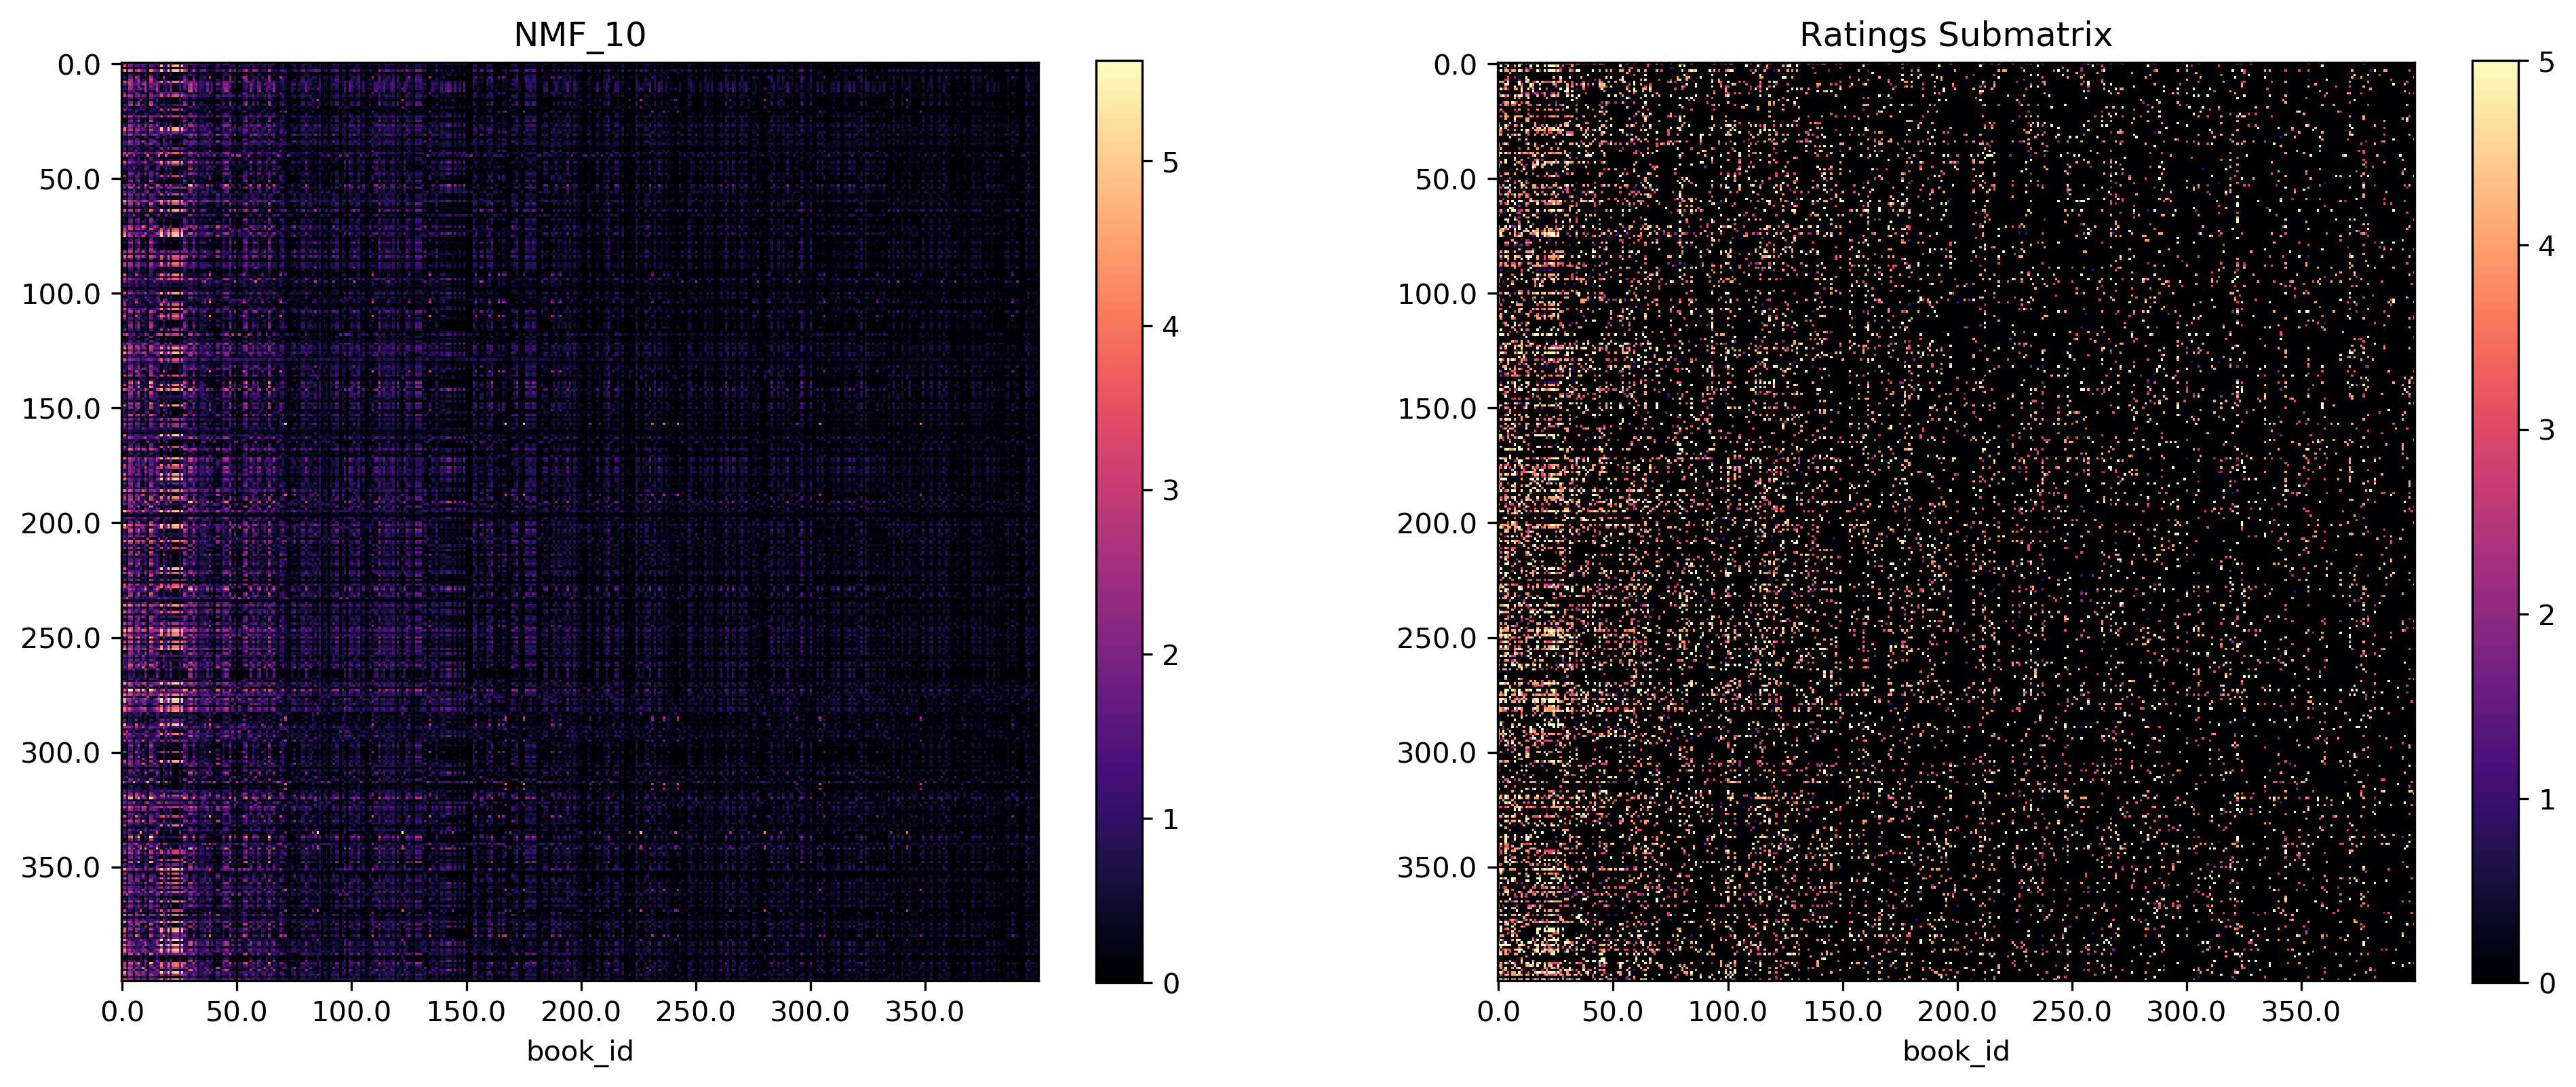
\includegraphics[width=\linewidth]{../image/goodreads-models/nmf-10-left.png}
%    \vspace{-30pt}
    \caption[NMF-10]{The matrix reconstruction ($k=10$).}
     \label{fig:nmf-1}
\end{figure}
\end{frame}

\subsection{$k=25$}\label{k-25}

\begin{frame}
 \begin{figure}[t]
  %  \centering
    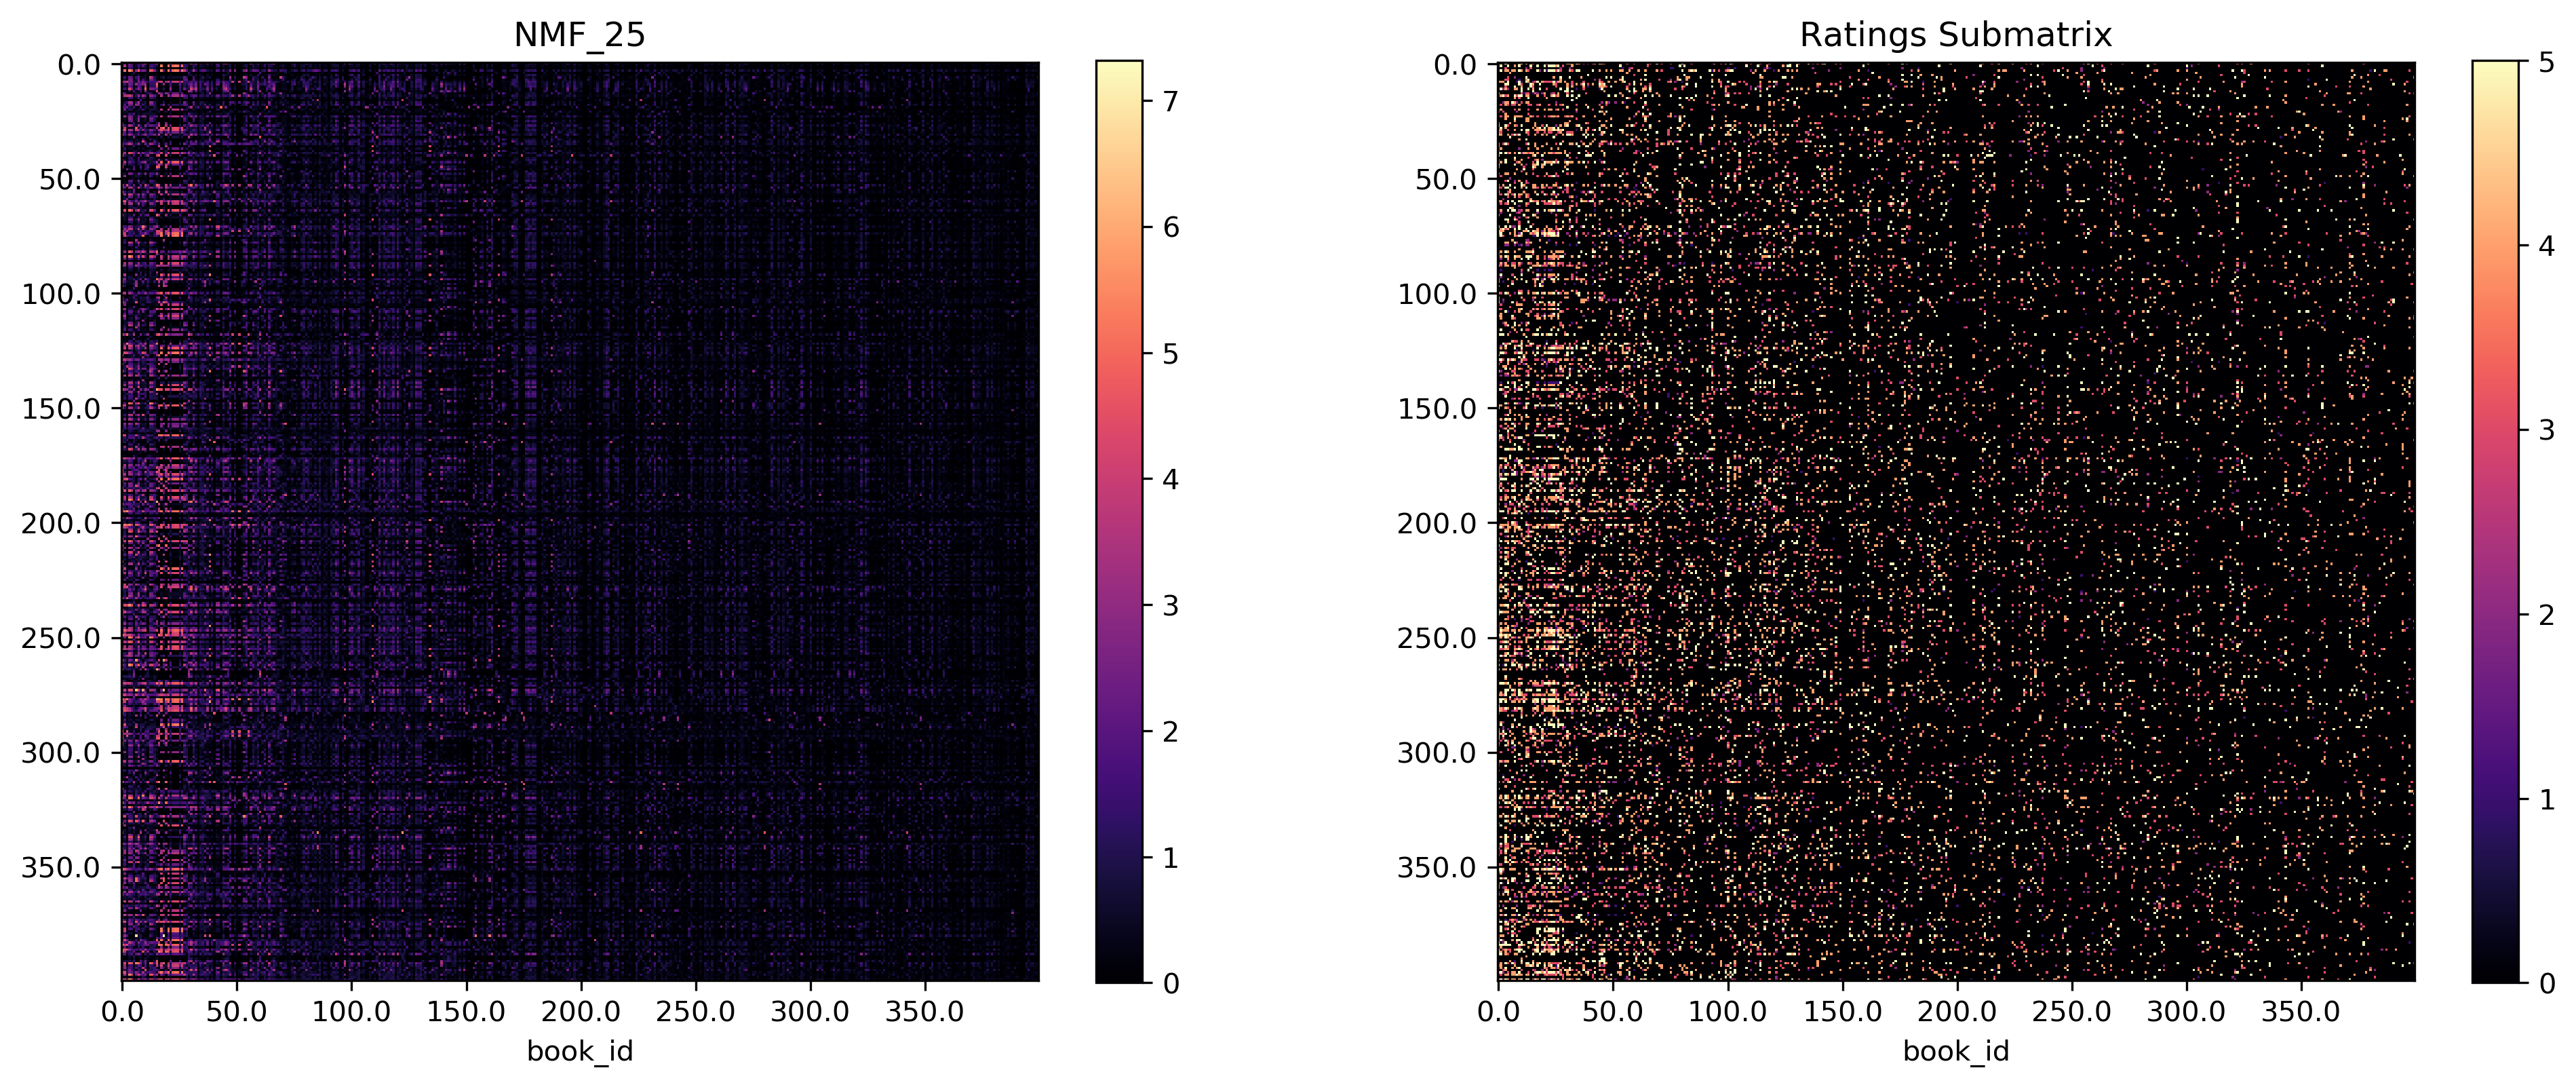
\includegraphics[width=\linewidth]{../image/goodreads-models/nmf-25-left.png}
%    \vspace{-30pt}
    \caption[NMF-25]{The matrix reconstruction ($k=25$).}
     \label{fig:nmf-25}
\end{figure}
\end{frame}


\subsection{$k=10$ Close}\label{k-10-close}



\begin{frame}
 \begin{figure}[t]
  %  \centering
    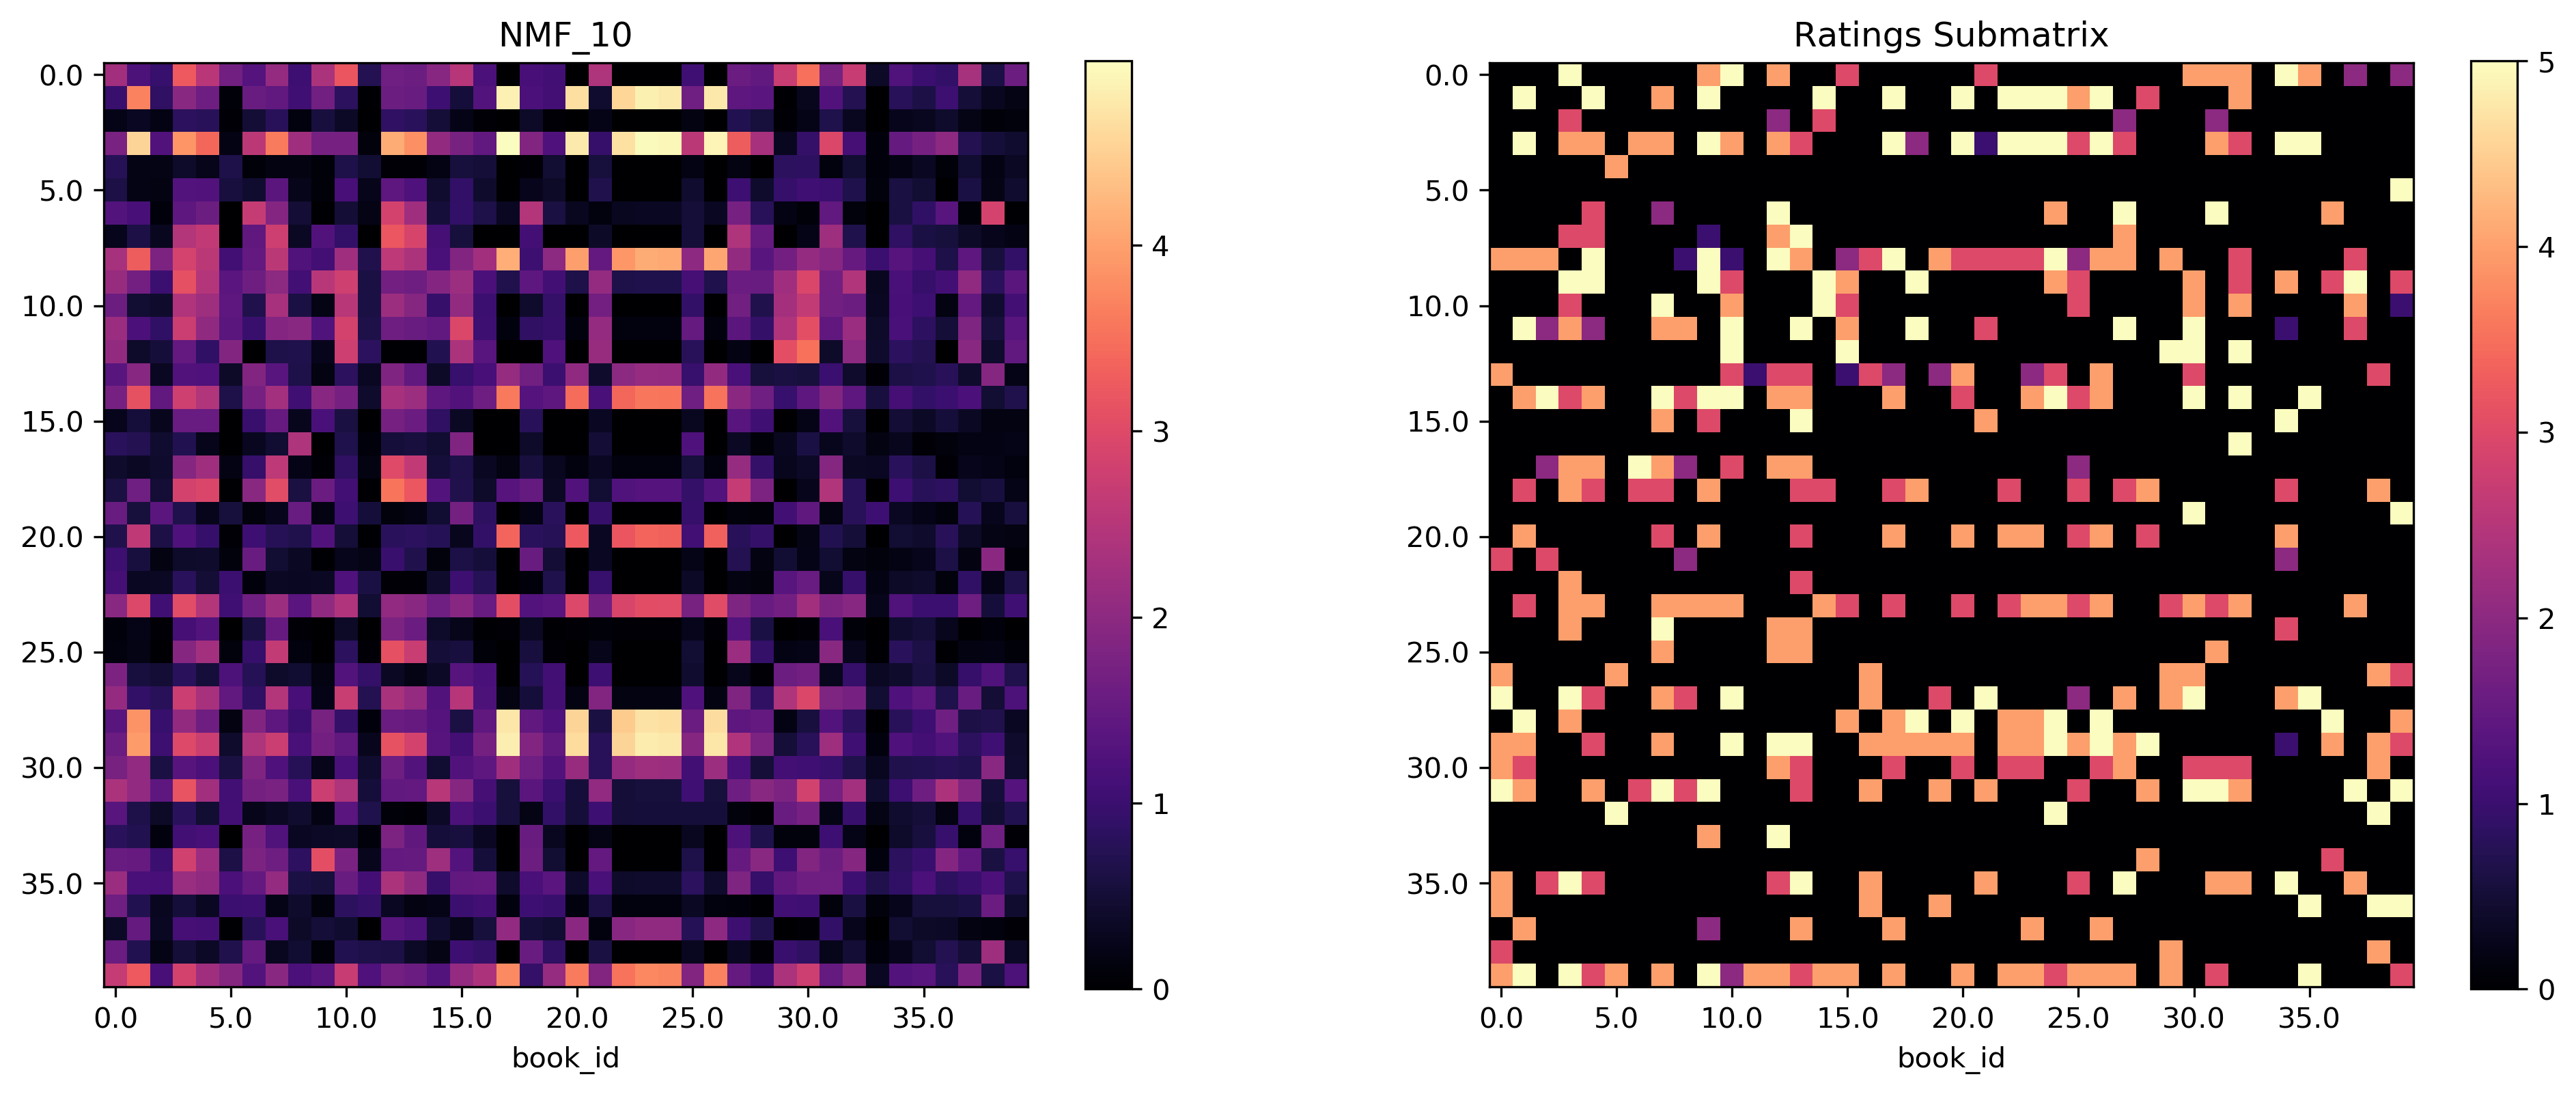
\includegraphics[width=\linewidth]{../image/goodreads-models/nmf-10-left-close.png}
%    \vspace{-30pt}
    \caption[NMF-10-left-close]{The matrix reconstruction ($k=10$).}
     \label{fig:nmf-10-left-close}
\end{figure}
\end{frame}

\subsection{$k=50$ Close}\label{k-50-close}

\begin{frame}
 \begin{figure}[t]
  %  \centering
    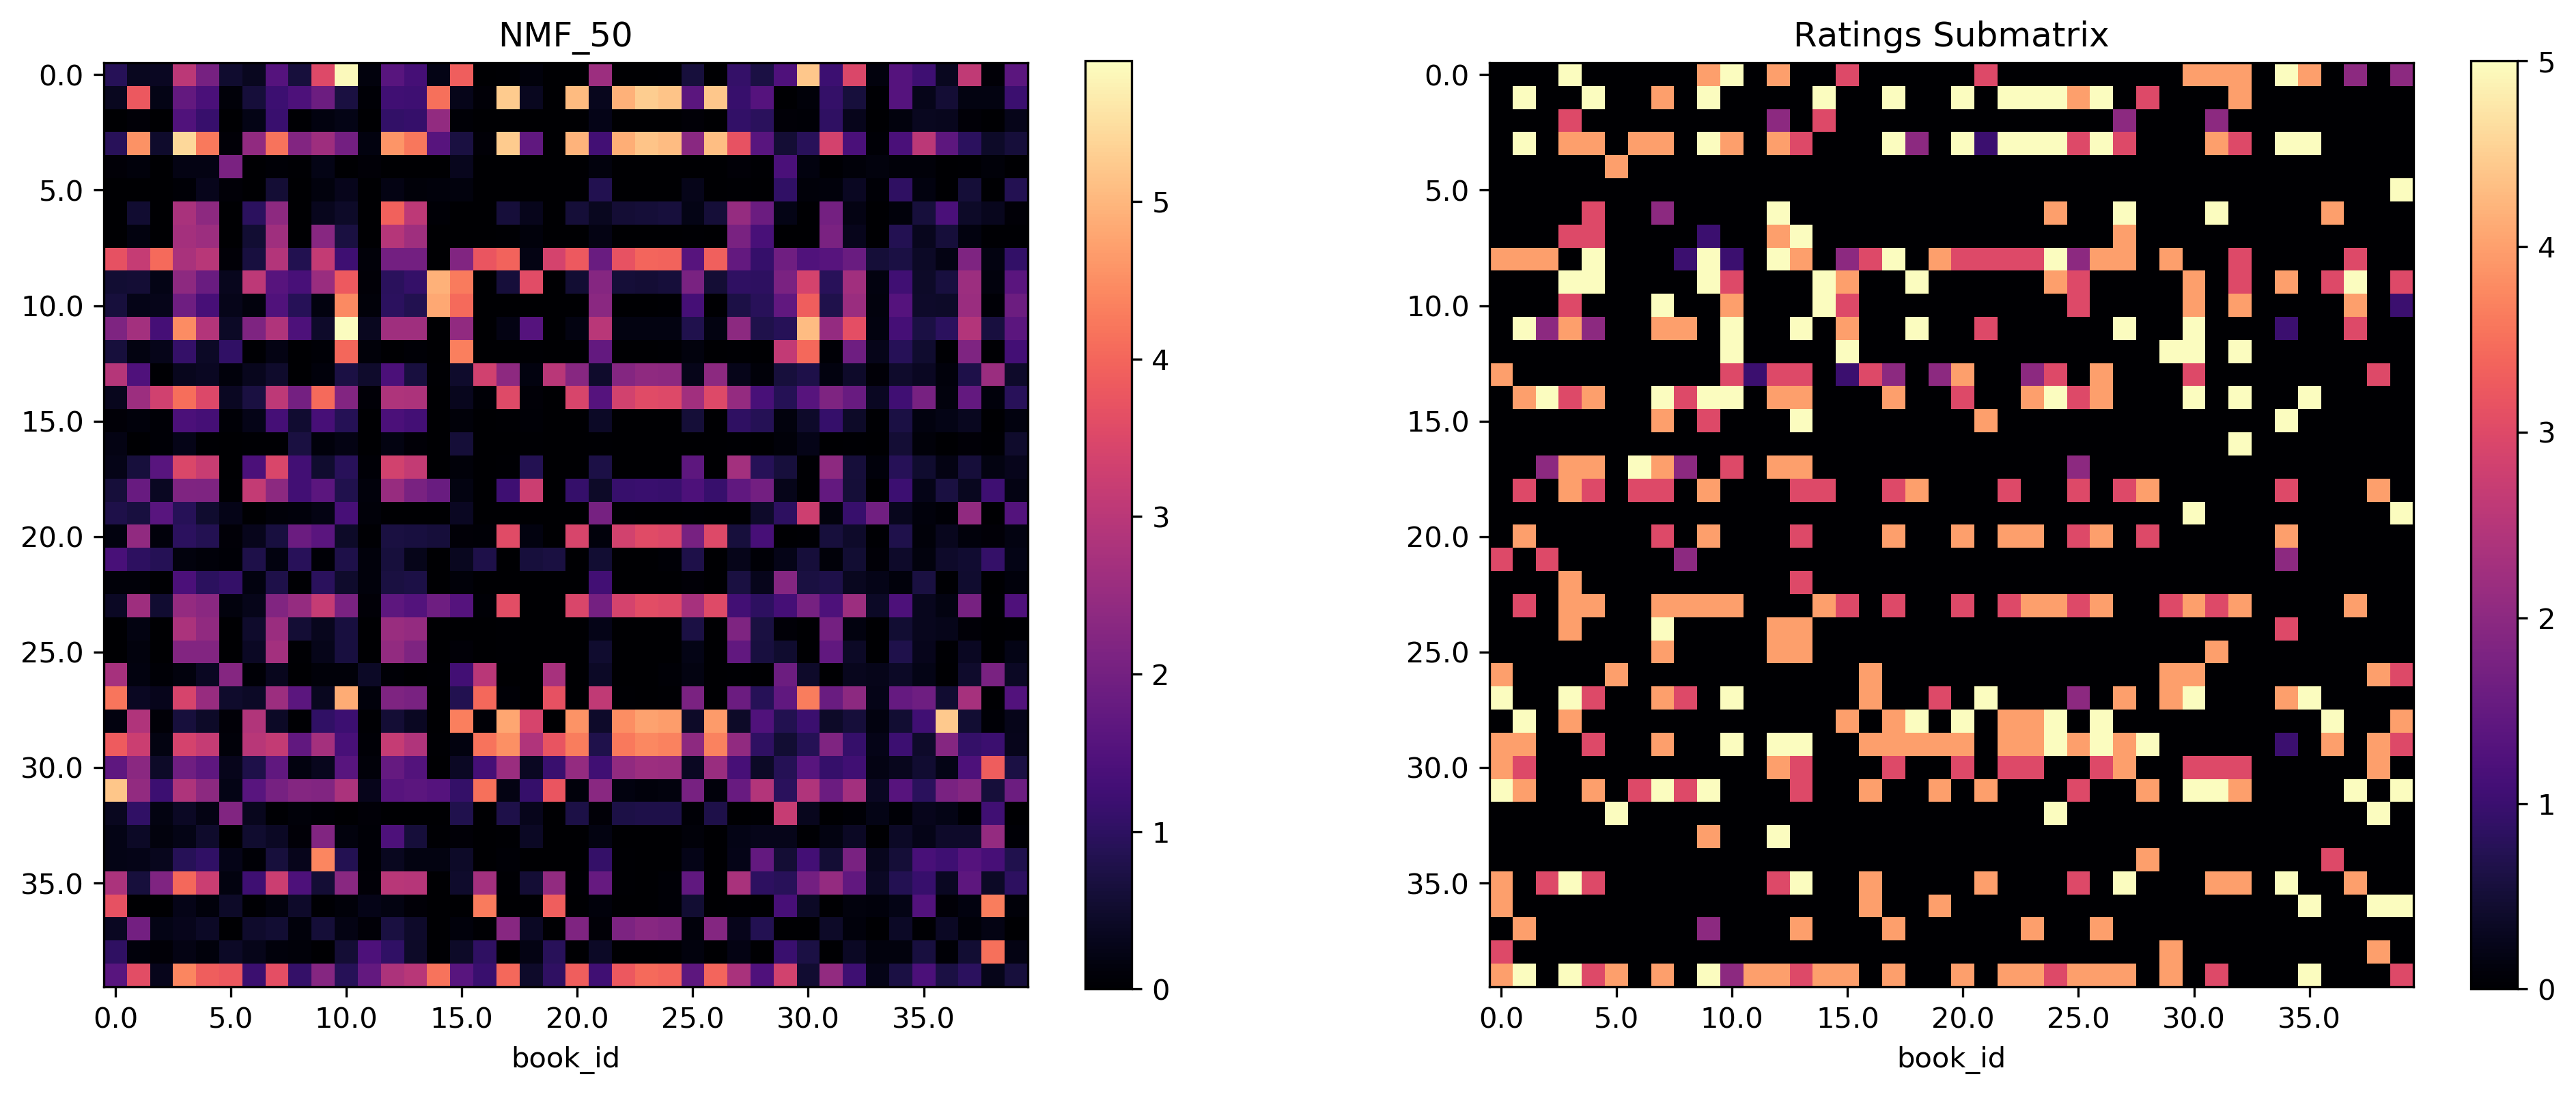
\includegraphics[width=\linewidth]{../image/goodreads-models/nmf-50-left-close.png}
%    \vspace{-30pt}
    \caption[NMF-50-left-close]{The matrix reconstruction ($k=50$).}
     \label{fig:nmf-50-left-close}
\end{figure}
\end{frame}

\subsection{$k=250$ Close}\label{k-250-close}

\begin{frame}
 \begin{figure}[t]
  %  \centering
    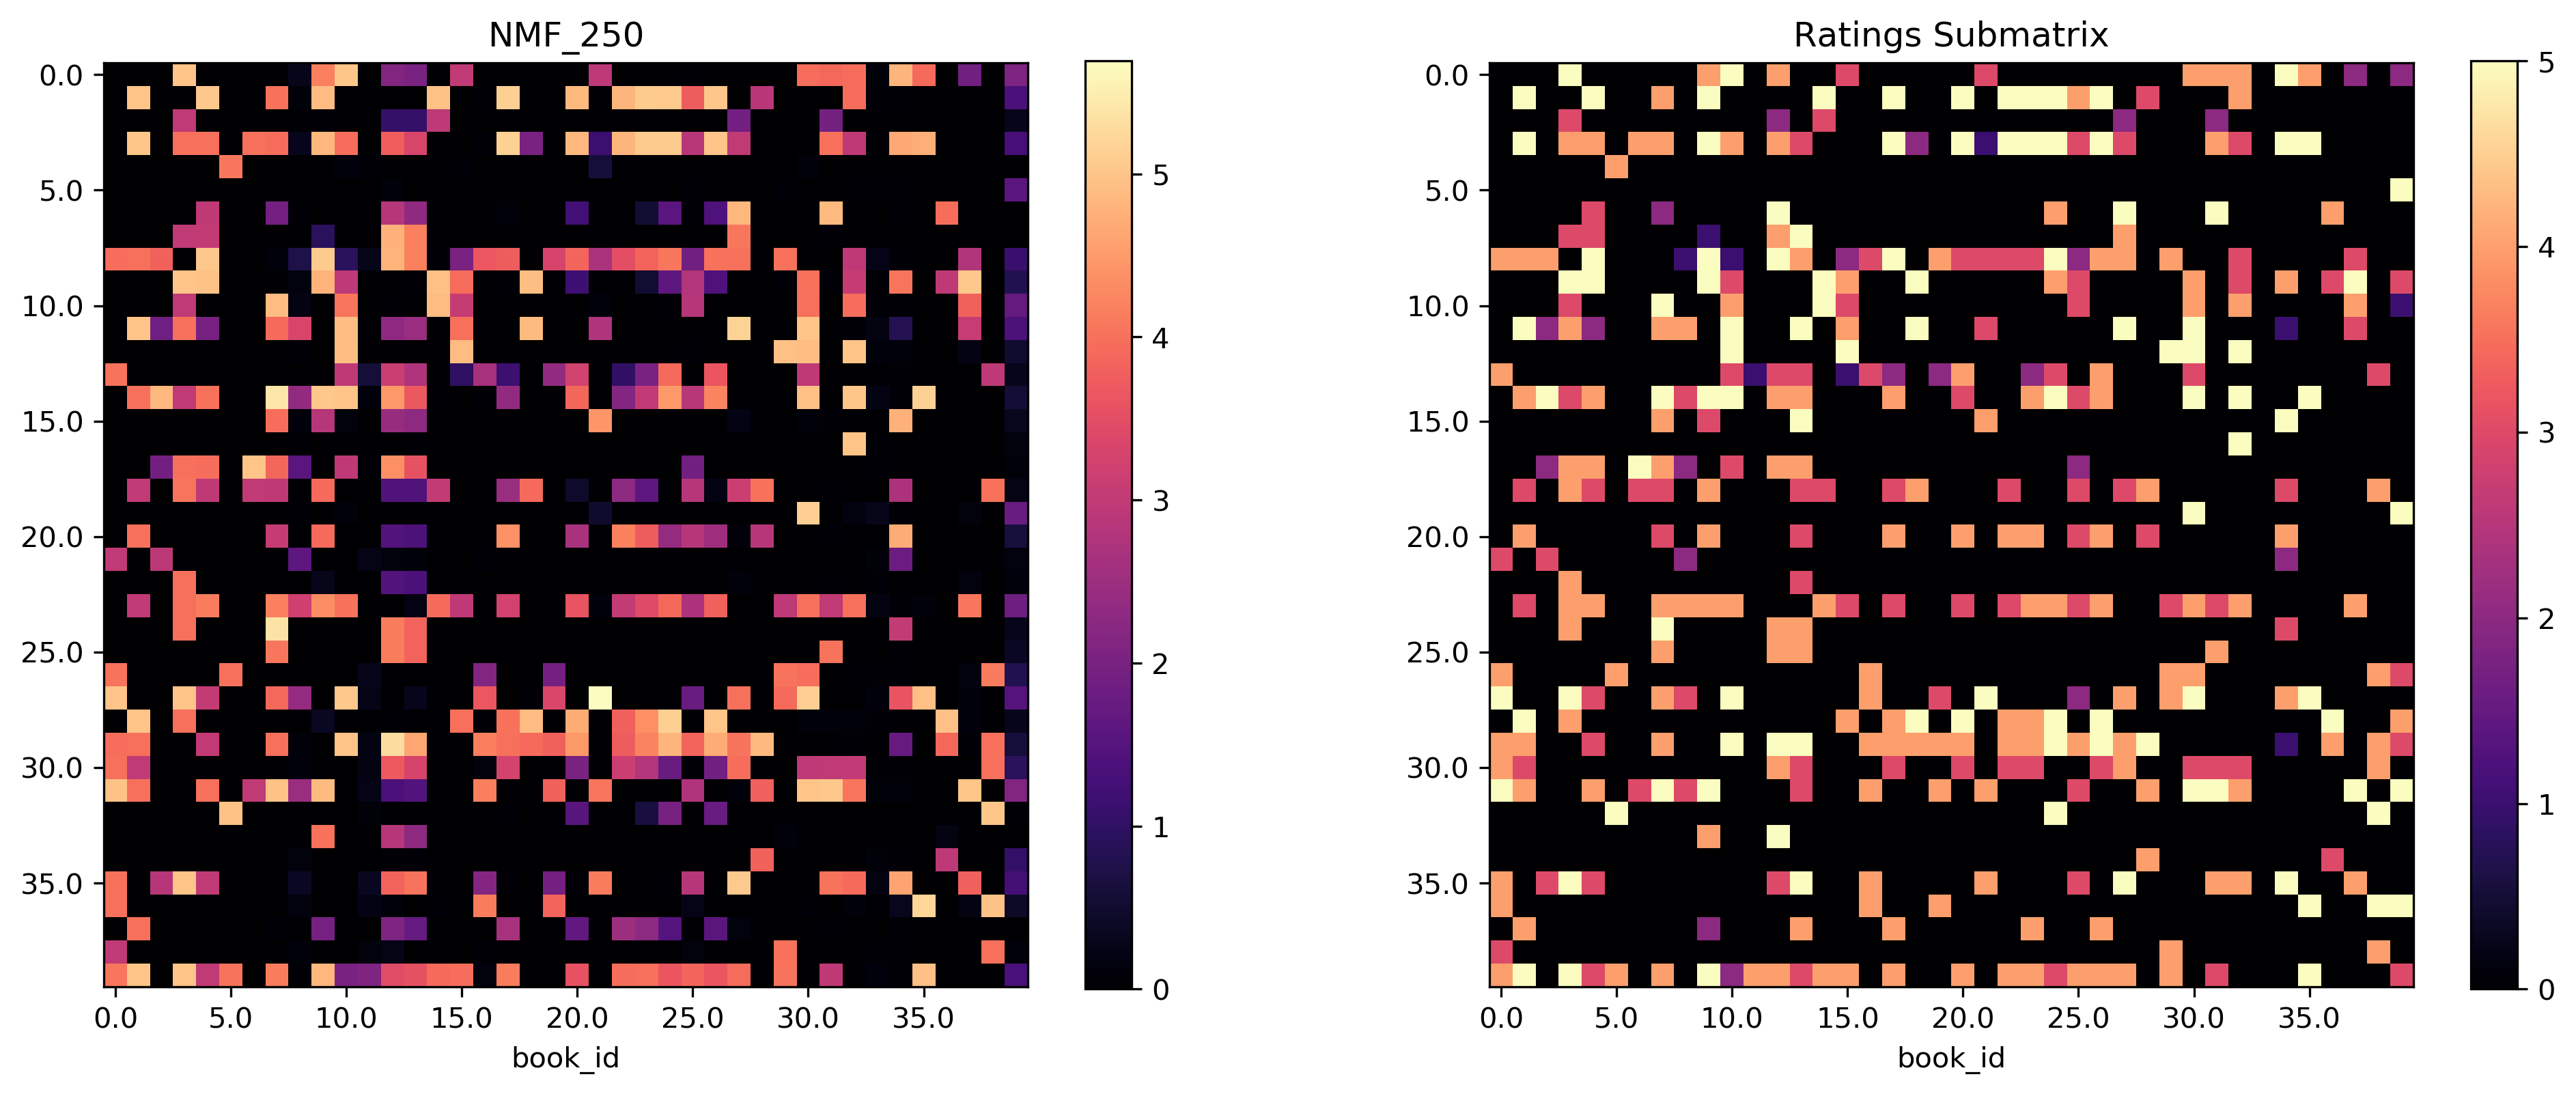
\includegraphics[width=\linewidth]{../image/goodreads-models/nmf-250-left-close.png}
%    \vspace{-30pt}
    \caption[NMF-250-left-close]{The matrix reconstruction ($k=250$).}
     \label{fig:nmf-250-left-close}
\end{figure}
\end{frame}

\subsection{$k=10$ Left Center Close}\label{k-10-left-center-close}


\begin{frame}
 \begin{figure}[t]
  %  \centering
    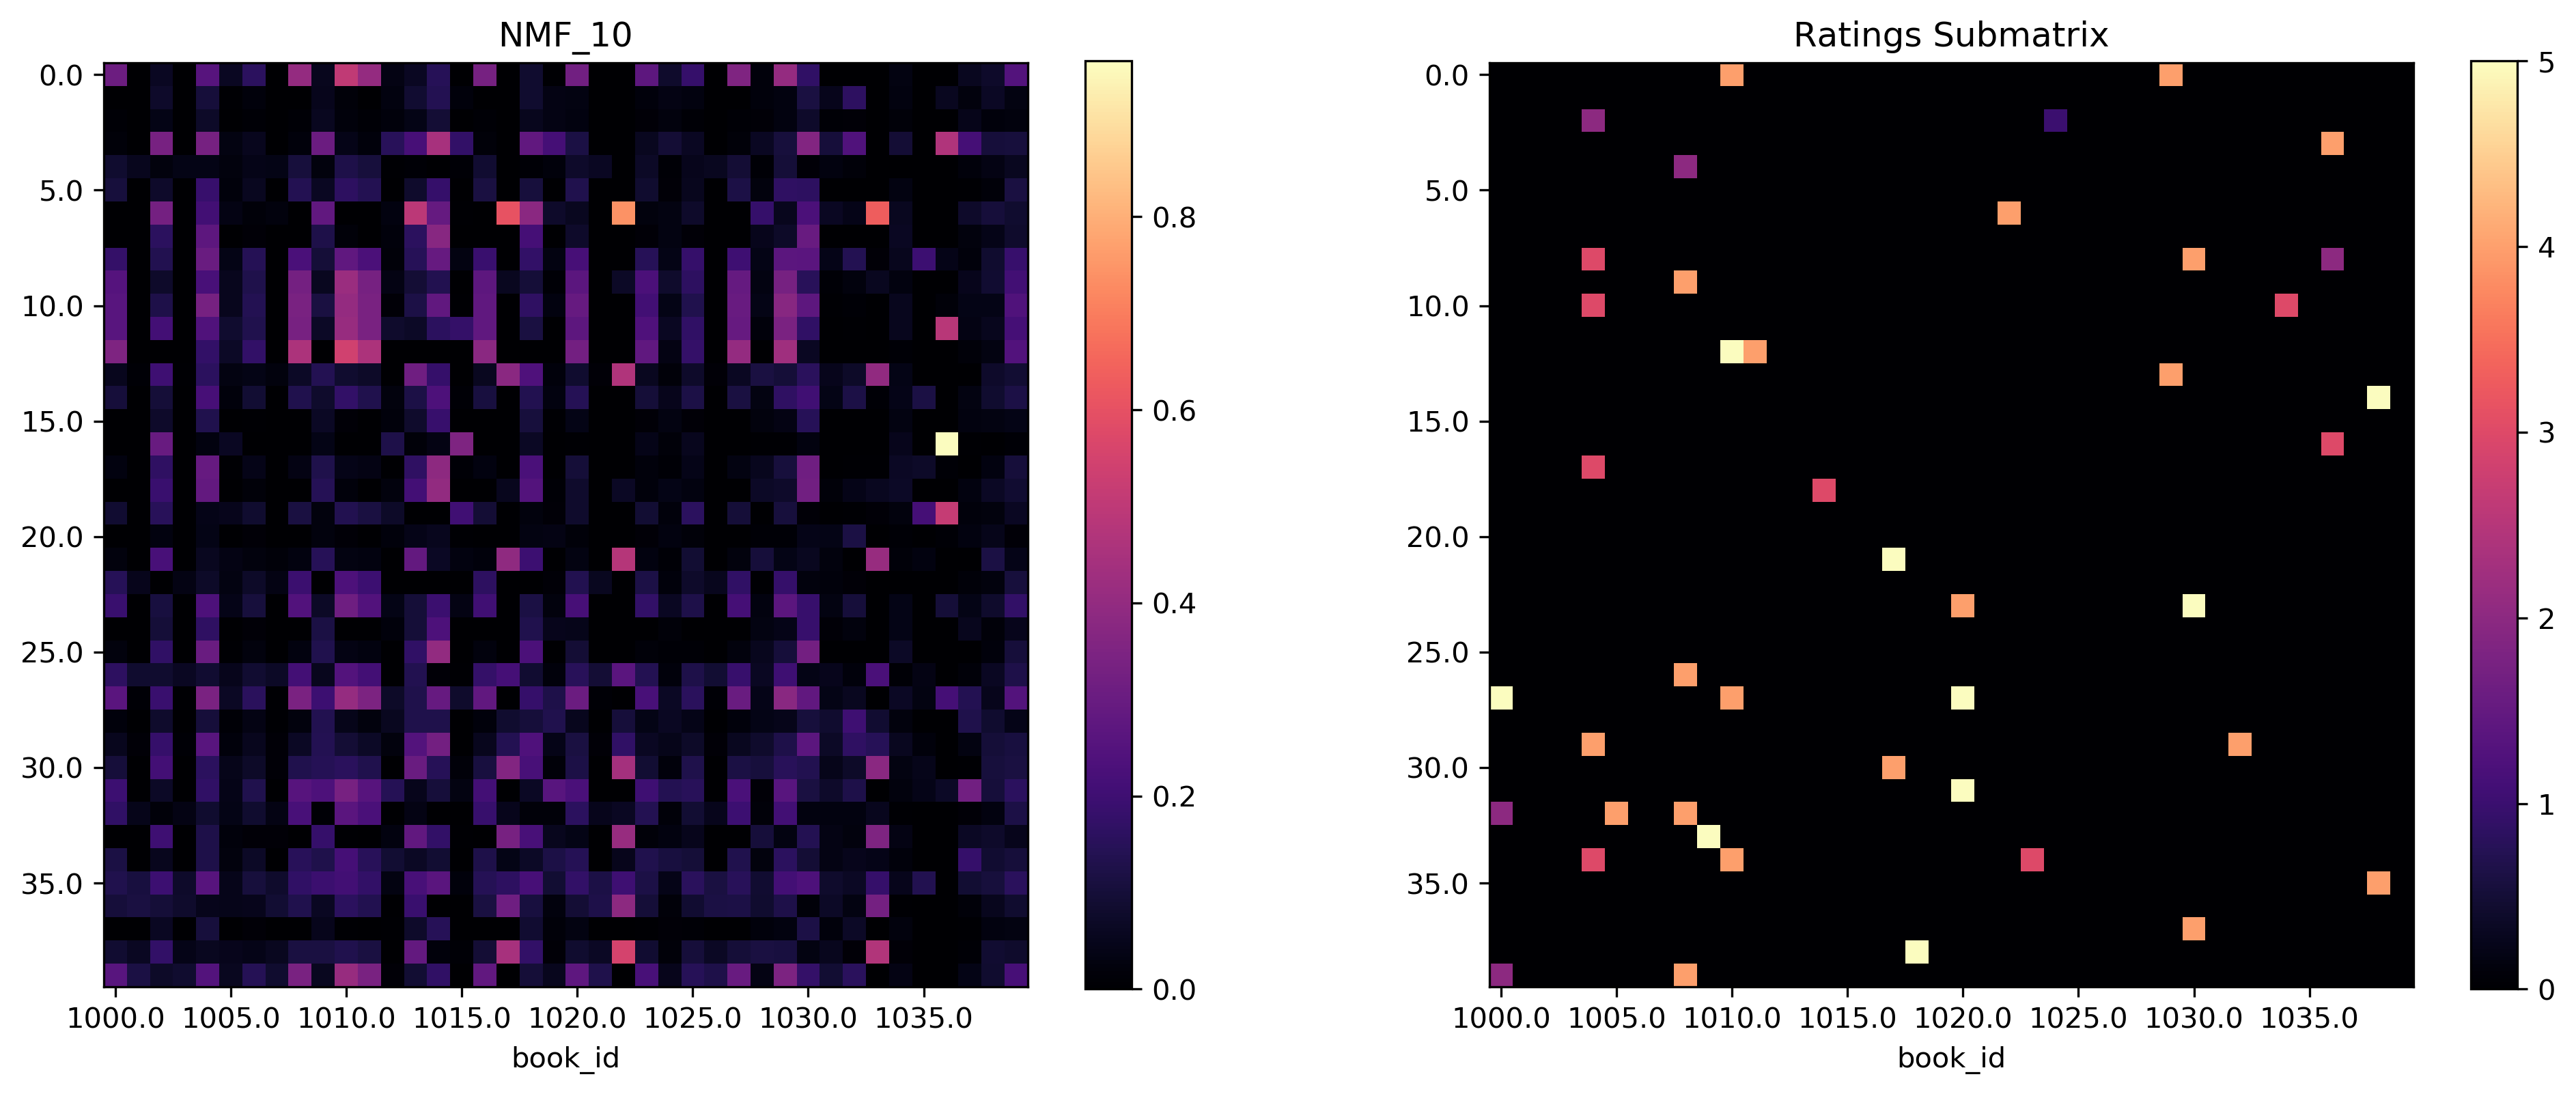
\includegraphics[width=\linewidth]{../image/goodreads-models/nmf-10-left-center-close.png}
%    \vspace{-30pt}
    \caption[NMF-10-left-center-close]{The matrix reconstruction ($k=10$).}
     \label{fig:nmf-10-left-center-close}
\end{figure}
\end{frame}

\subsection{$k=50$ Left Center Close}\label{k-50-left-center-close}

\begin{frame}
 \begin{figure}[t]
  %  \centering
    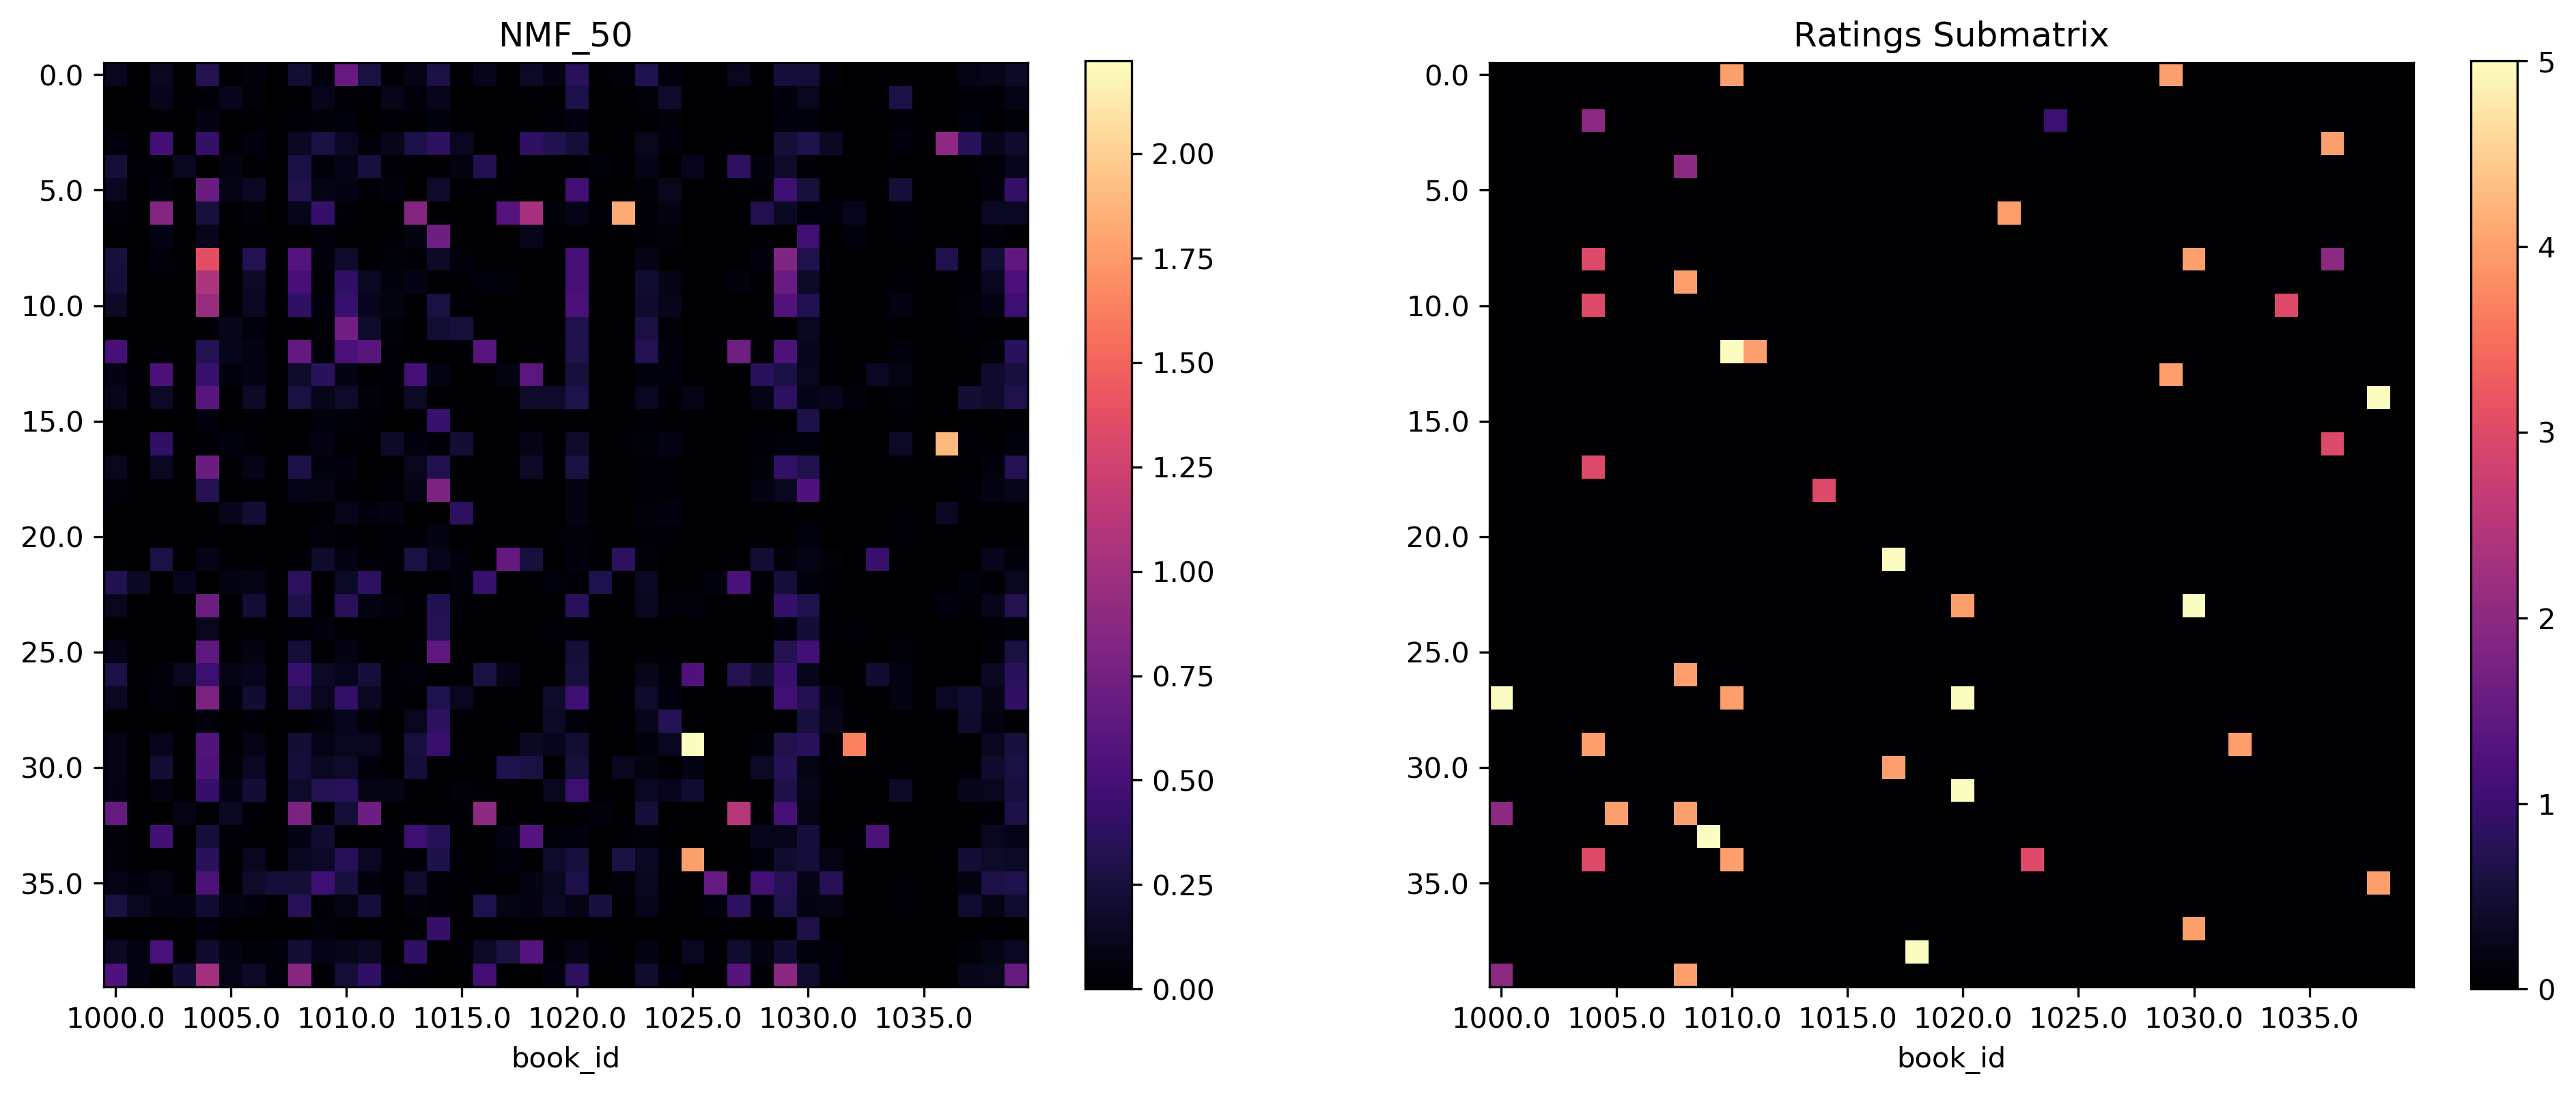
\includegraphics[width=\linewidth]{../image/goodreads-models/nmf-50-left-center-close.png}
%    \vspace{-30pt}
    \caption[NMF-50-left-center-close]{The matrix reconstruction ($k=50$).}
     \label{fig:nmf-50-left-center-close}
\end{figure}
\end{frame}

\subsection{$k=250$ Left Center Close}\label{k-250-left-center-close}

\begin{frame}
 \begin{figure}[t]
  %  \centering
    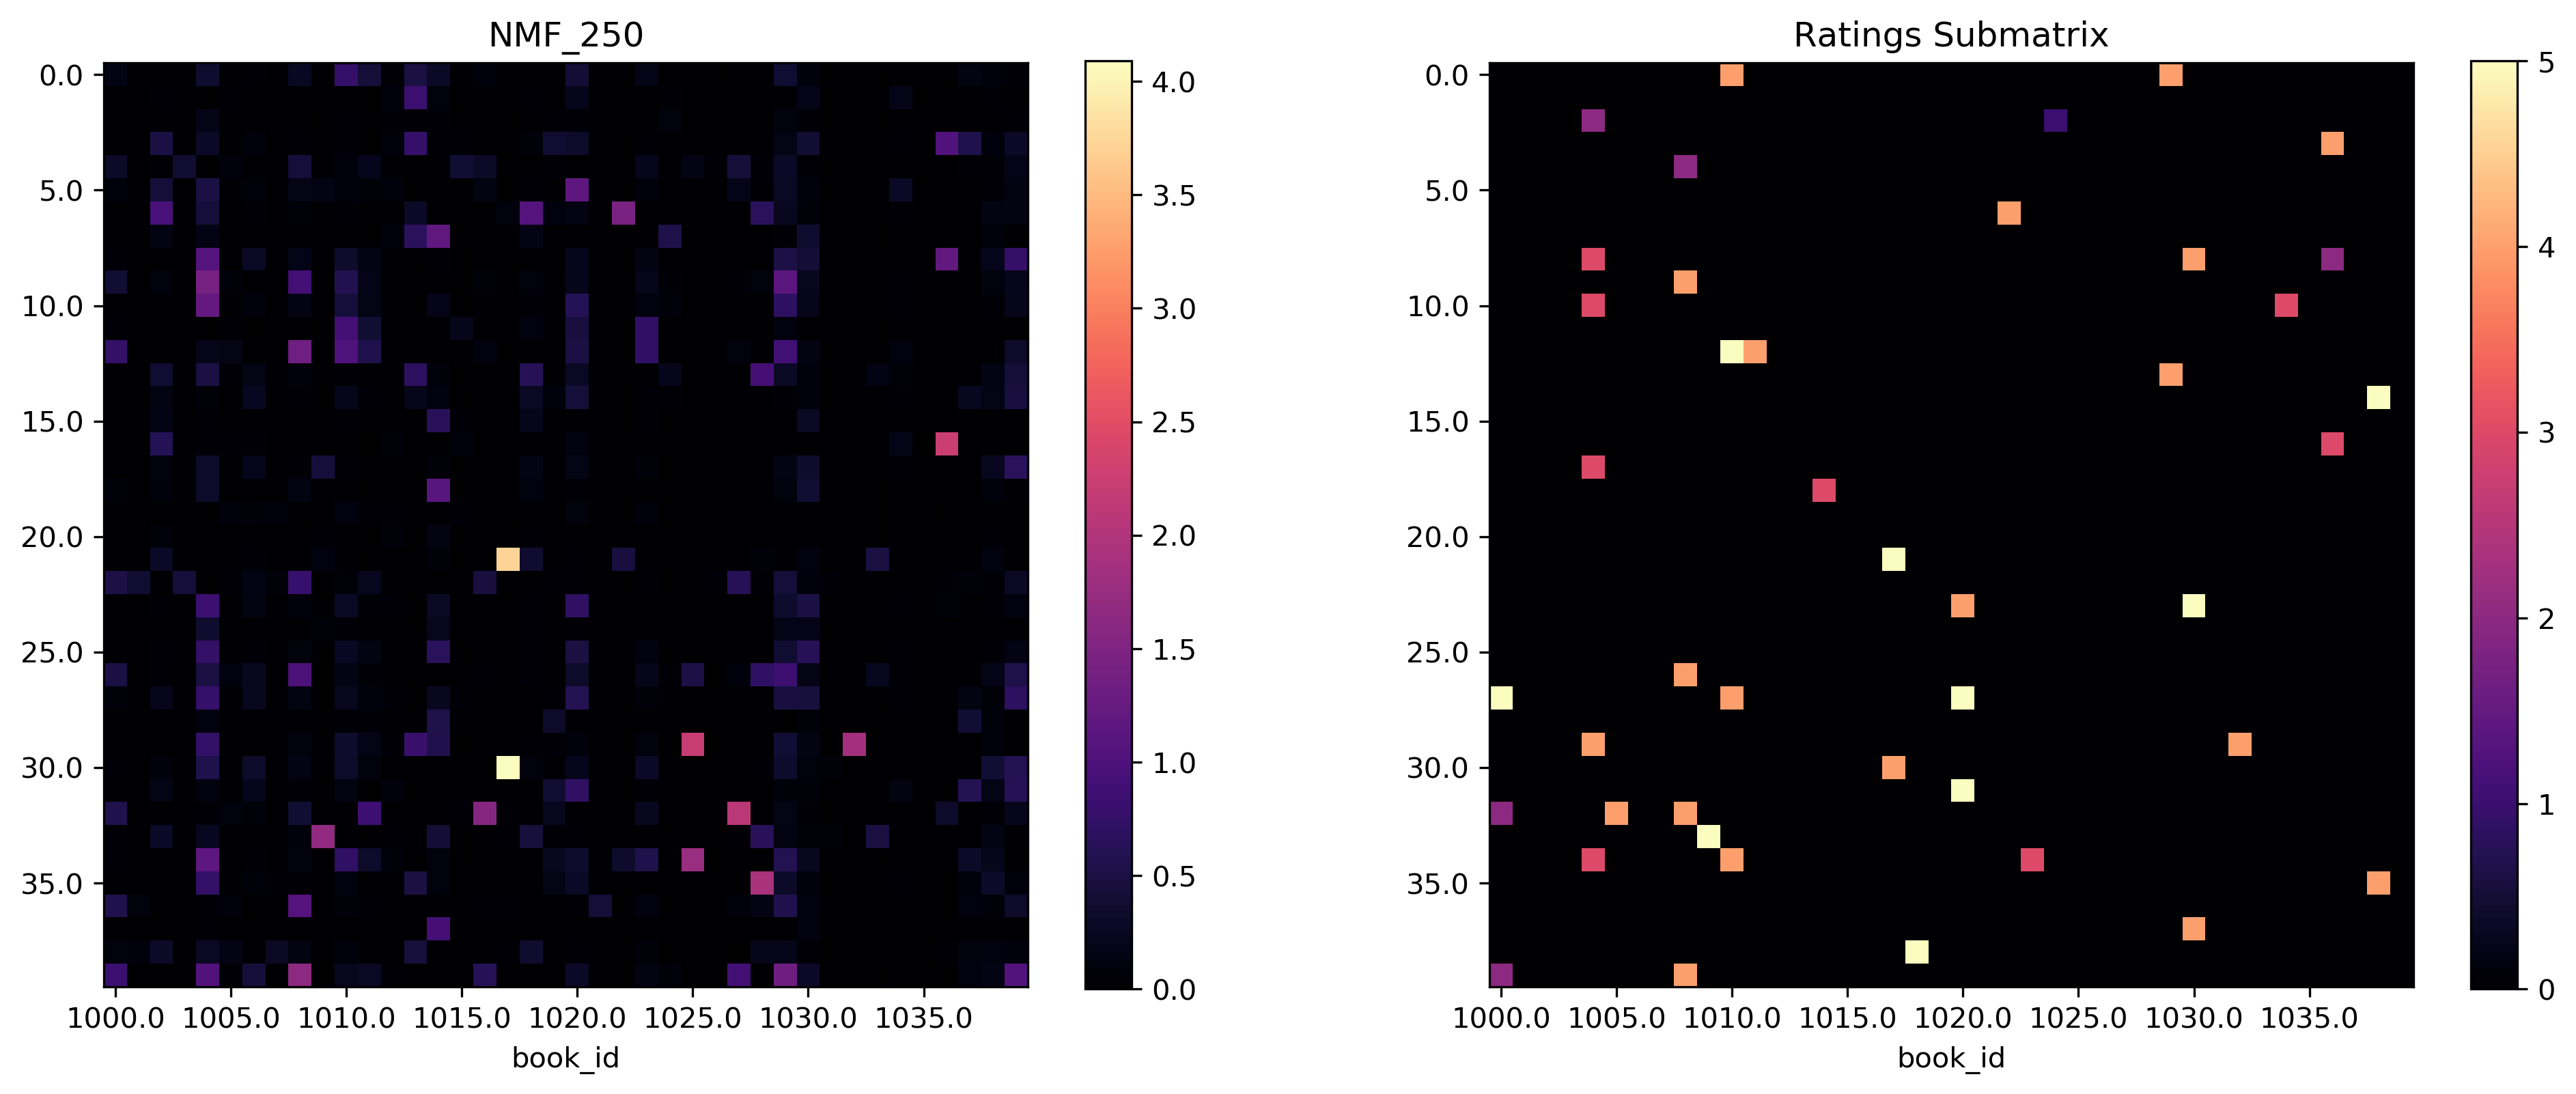
\includegraphics[width=\linewidth]{../image/goodreads-models/nmf-250-left-center-close.png}
%    \vspace{-30pt}
    \caption[NMF-250-left-center-close]{The matrix reconstruction ($k=250$).}
     \label{fig:nmf-250-left-center-close}
\end{figure}
\end{frame}

\subsection{Scores}\label{scores}

\begin{frame}
 
\begin{figure}[h]
  %  \centering
    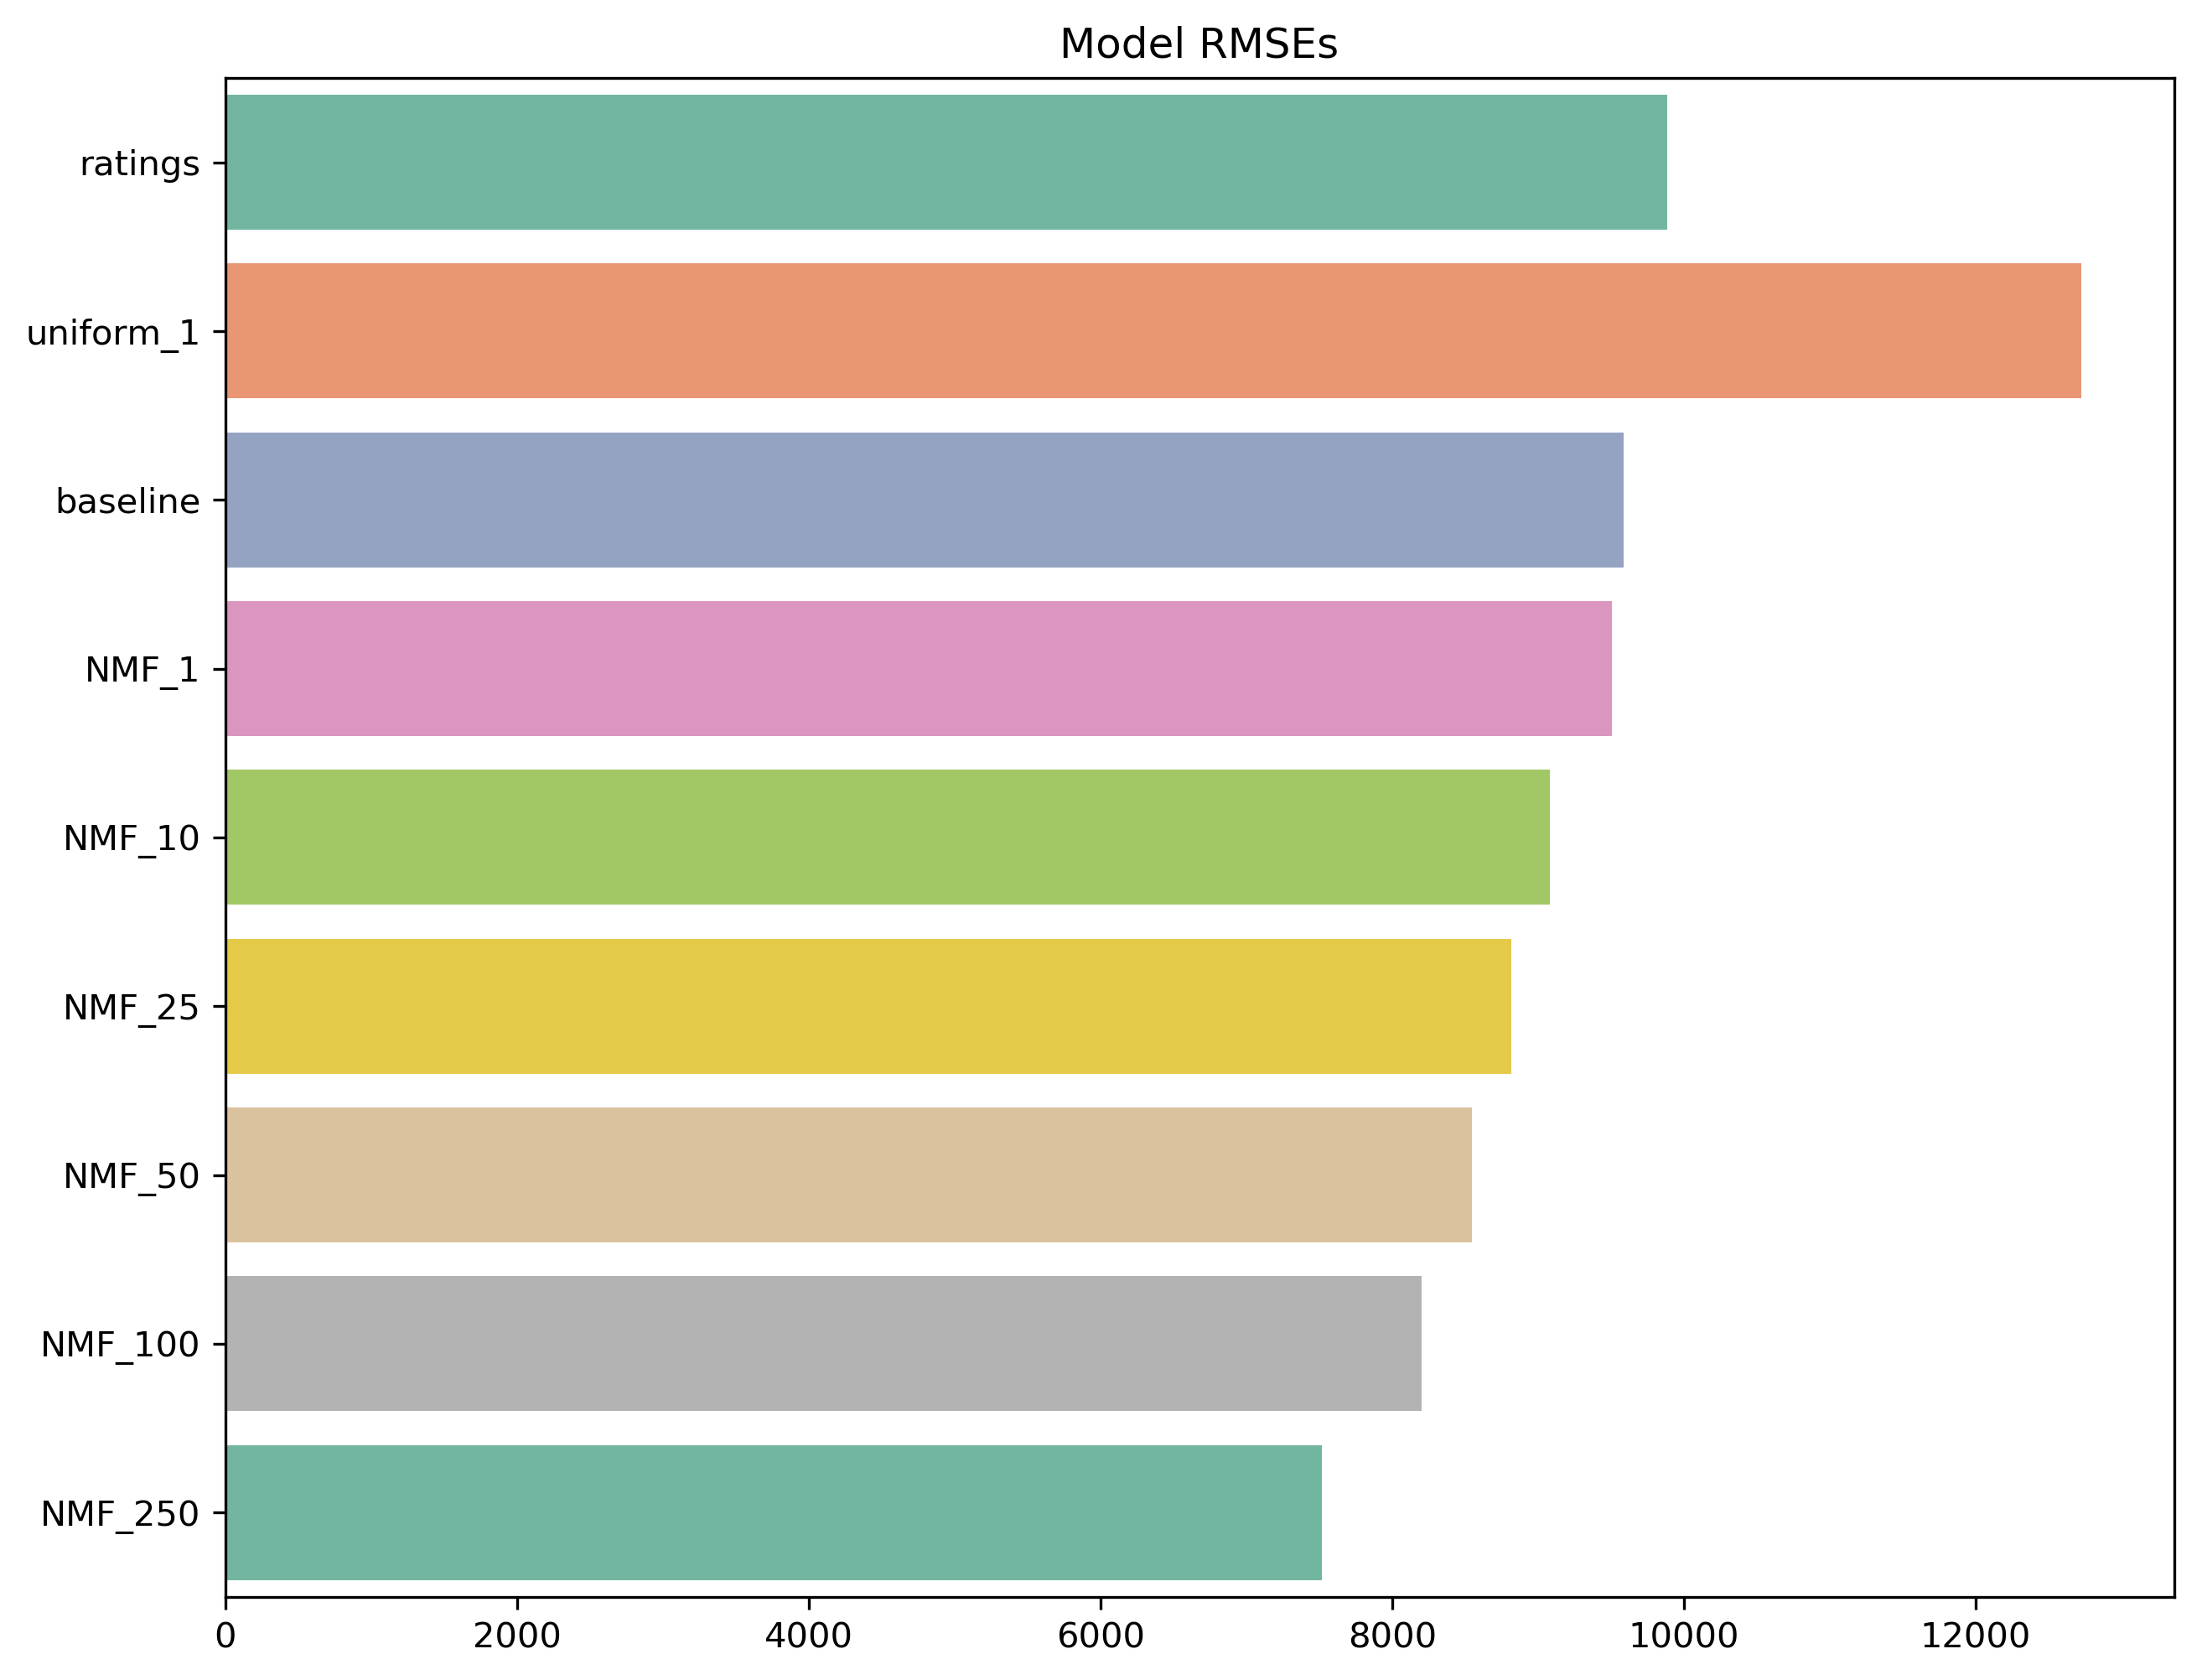
\includegraphics[width=0.8\linewidth]{../image/goodreads-models/model-rmses.png}
%    \vspace{-30pt}
    \caption[RMSE Comparison]{RMSE scores for each model.}
     \label{fig:rmse}
\end{figure}
\end{frame}

\section{Applications}

\subsection{Topics ($k=10$)}

\begin{frame}
 \begin{figure}[t]
    \centering
    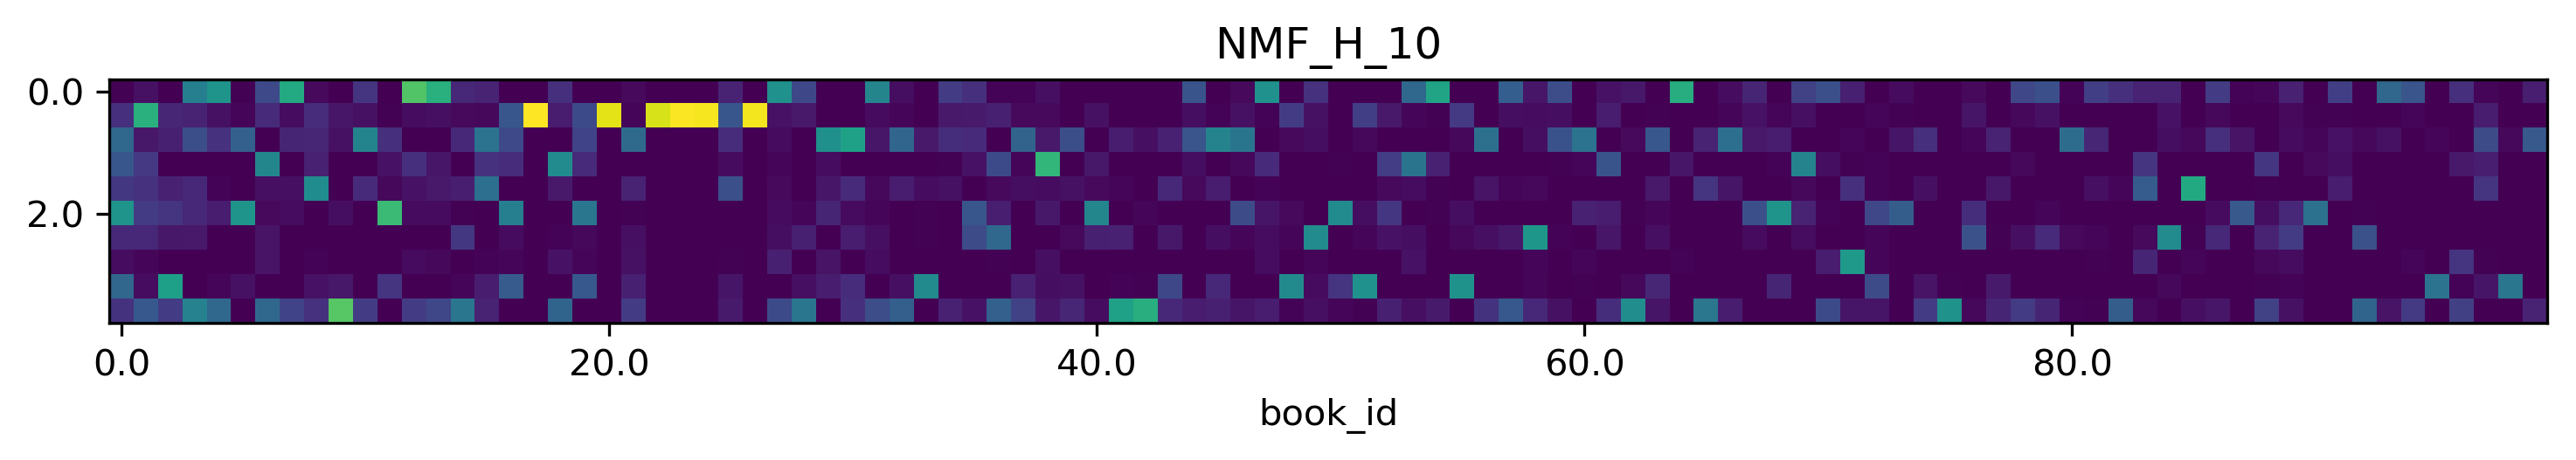
\includegraphics[width=\textwidth, trim=3cm 0cm 0cm 0cm, clip]{../image/goodreads-models/nmf-H-10.png}
%    \vspace{-30pt}
    \caption[NMF-H-10]{The \emph{book preferenced matrix} $H$ ($k=10$).}
     \label{fig:nmf-H-10}
\end{figure}

\begin{columns}
\column{0.65\textwidth}
\begin{itemize}[<+->]
\item Rows $h^\ell$ of $H$ indicate book correlation with latent topic $\ell$.\vfill
\item Components of $h^\ell$ are weights for tags:\vfill
\begin{itemize}[<+->]
\item We have the count $n_{b,t}$ of the top 100 tags for each book\vfill
\item The \emph{tag frequency} $r^\ell_t$ for tag $t$ in latent factor $\ell$ is $\displaystyle r_t^\ell = \sum_{b} h^\ell_b n_{b,t}.$
\end{itemize}
\end{itemize}
\column{0.35\textwidth}
%______________________________________________________________________
\begin{figure}
\vspace{-20pt}
\centering
  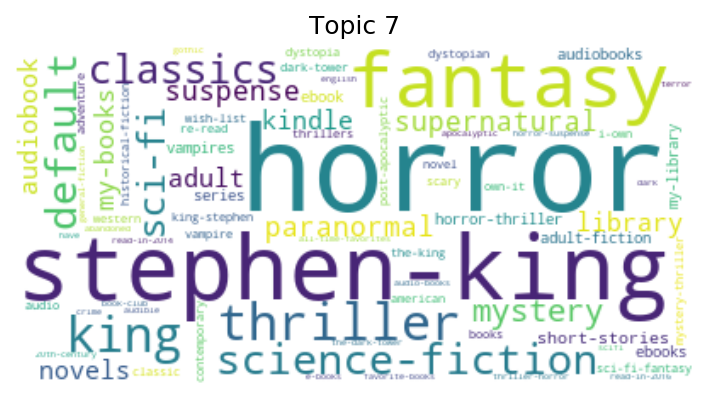
\includegraphics[width=\linewidth]{../image/goodreads-topics-profiles-recommendations/tag-cloud-10-7.png}
  \caption[Tag Cloud for Topic 7 ($k=10$)]{Tag cloud for topic 7 ($k=10$).}
  \label{fig:tag-cloud-10-7}
%  \vspace{-30pt}
\end{figure}
%______________________________________________________________________
\end{columns}

\vfill
\end{frame}

\begin{frame}

\begin{table}
\centering
\begin{tabular}{ll}
\toprule
                        authors &                                title \\
\midrule
                   Stephen King &                                   It \\
 Stephen King, \ldots%Bernie Wrightson 
 &                            The Stand \\
                   Stephen King &         The Shining (The Shining \#1) \\
                   Stephen King &                               Misery \\
                   Stephen King &                               Carrie \\
                   Stephen King &                         Pet Sematary \\
                   Stephen King &                         'Salem's Lot \\
                   Stephen King &                       Needful Things \\
                   Stephen King &  The Gunslinger (The Dark Tower, \#1)
                    \\
                   Stephen King &                       The Green Mile \\
                   Stephen King &                        The Dead Zone \\
                   Stephen King &                          Firestarter \\
\bottomrule
\end{tabular}
  \caption[Stephen King ($k=10$)]{The top-scoring books in topic 7 ($k=10$) are all Stephen King.}
  \label{tab:stephen-king-10}
\end{table}



\end{frame}


\begin{frame}
\centering
  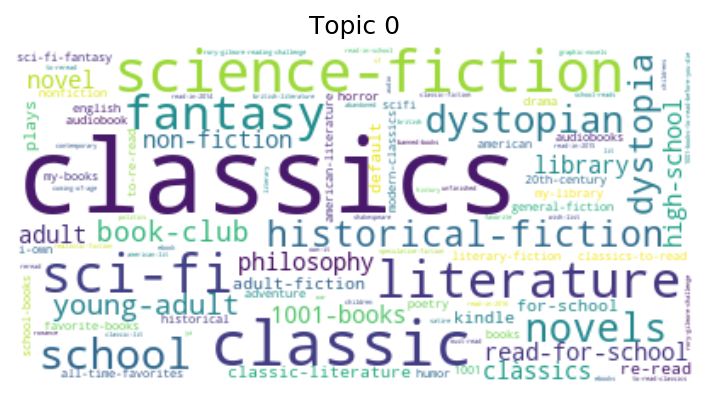
\includegraphics[width=0.45\textwidth]{../image/goodreads-topics-profiles-recommendations/tag-cloud-10-0.png} \hfill
    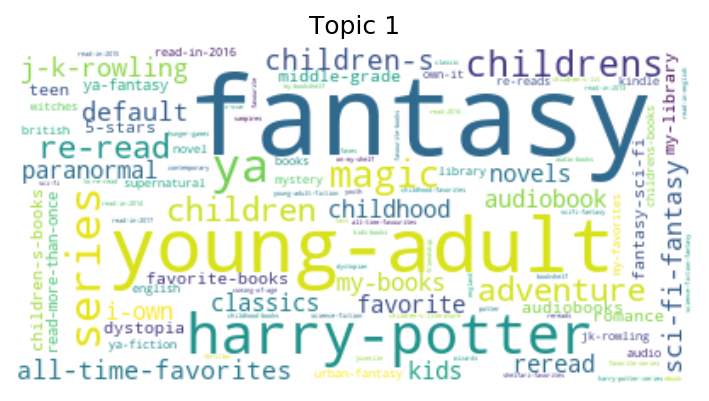
\includegraphics[width=0.45\textwidth]{../image/goodreads-topics-profiles-recommendations/tag-cloud-10-1.png}
    \vfill
    
      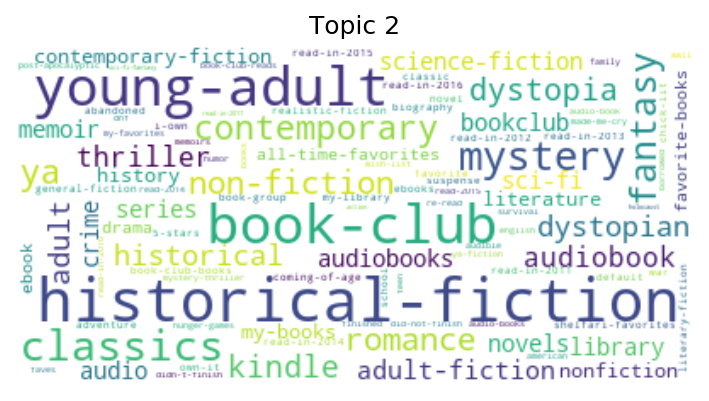
\includegraphics[width=0.45\textwidth]{../image/goodreads-topics-profiles-recommendations/tag-cloud-10-2.png} \hfill
        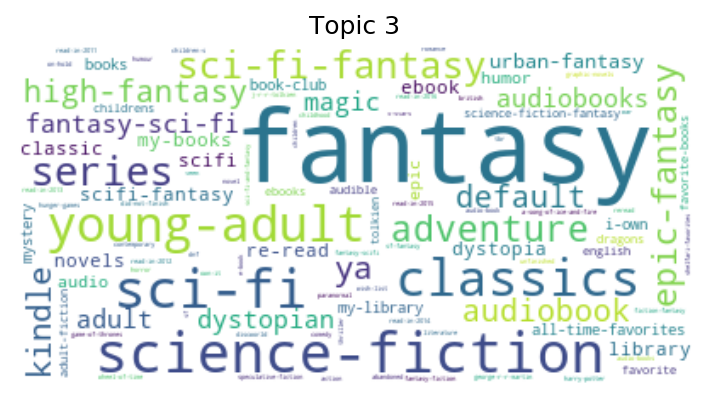
\includegraphics[width=0.45\textwidth]{../image/goodreads-topics-profiles-recommendations/tag-cloud-10-3.png}
\end{frame}

\begin{frame}
\centering
  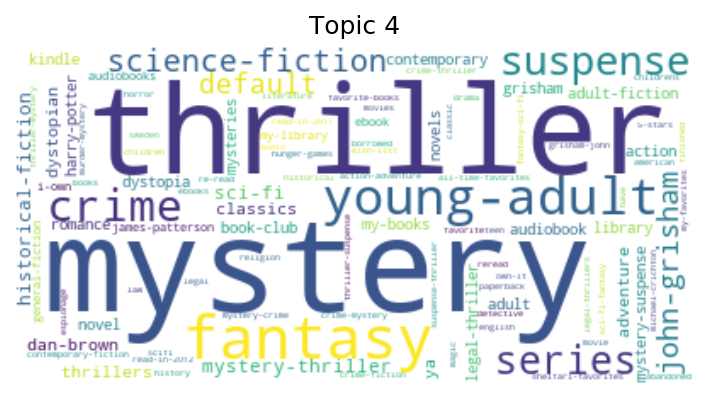
\includegraphics[width=0.45\textwidth]{../image/goodreads-topics-profiles-recommendations/tag-cloud-10-4.png} \hfill
    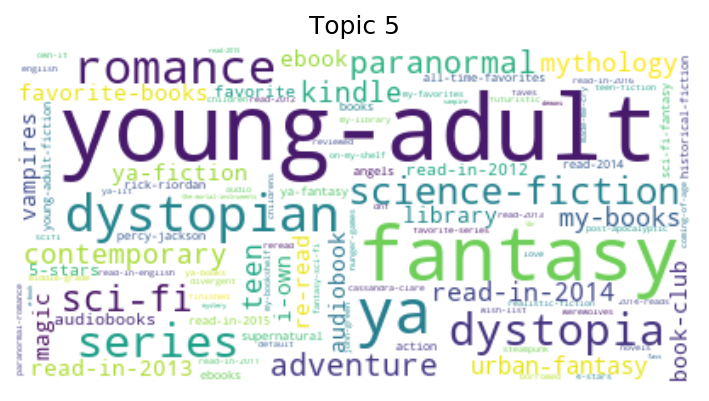
\includegraphics[width=0.45\textwidth]{../image/goodreads-topics-profiles-recommendations/tag-cloud-10-5.png}
    \vfill
    
      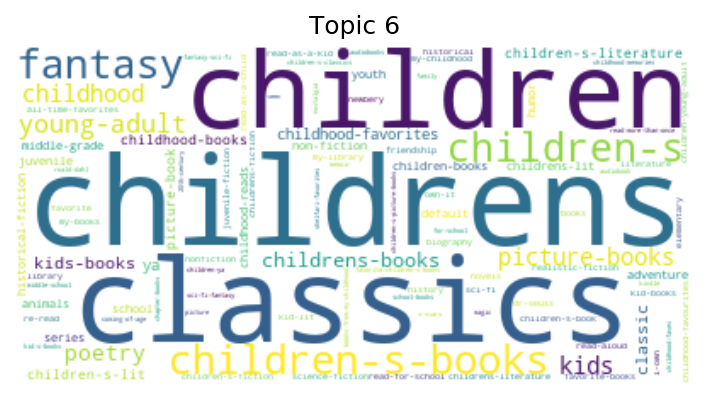
\includegraphics[width=0.45\textwidth]{../image/goodreads-topics-profiles-recommendations/tag-cloud-10-6.png} \hfill
        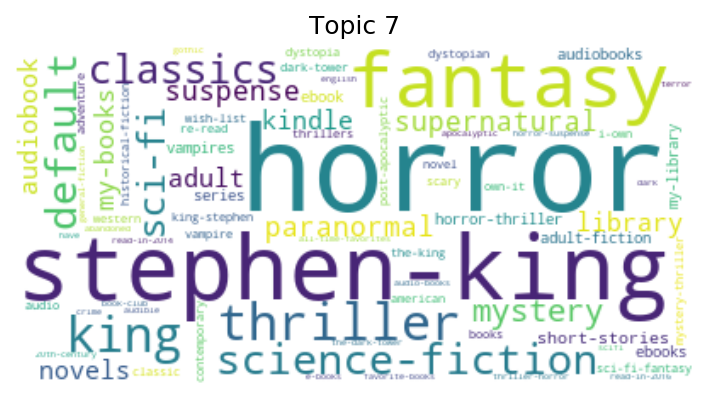
\includegraphics[width=0.45\textwidth]{../image/goodreads-topics-profiles-recommendations/tag-cloud-10-7.png}
\end{frame}

\begin{frame}
\centering
    \vfill
      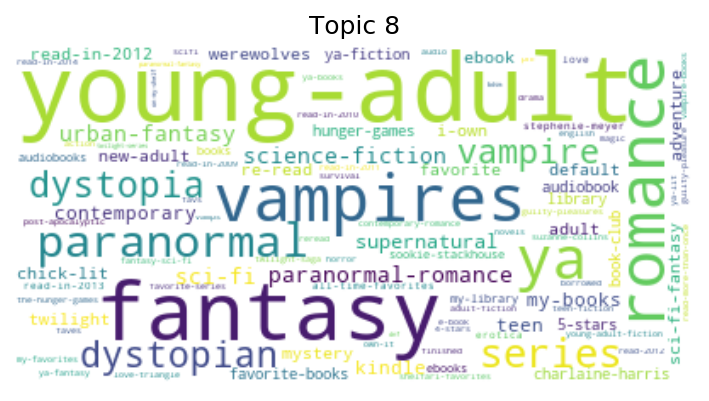
\includegraphics[width=0.45\textwidth]{../image/goodreads-topics-profiles-recommendations/tag-cloud-10-8.png} \hfill
    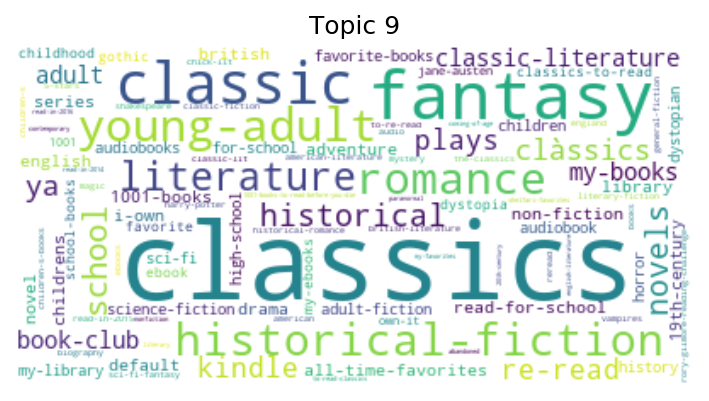
\includegraphics[width=0.45\textwidth]{../image/goodreads-topics-profiles-recommendations/tag-cloud-10-9.png}
    \vfill

\end{frame}



\subsection{Topics ($k=25$)}

\begin{frame}
 The topics are finer for greater latent factors $k$. When $k=25$ there are two distinct Stephen King topics: 
 
 \begin{figure}
%\vspace{-20pt}
\centering
  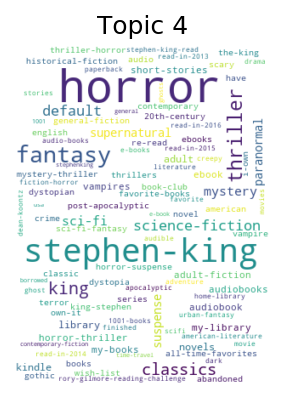
\includegraphics[width=0.45\linewidth]{../image/goodreads-topics-profiles-recommendations/tag-cloud-25-tall-4.png}
    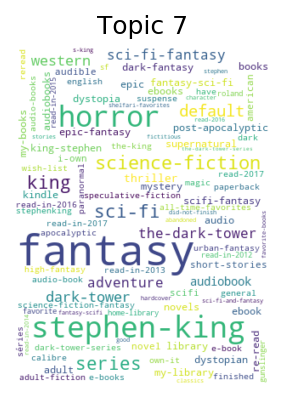
\includegraphics[width=0.45\linewidth]{../image/goodreads-topics-profiles-recommendations/tag-cloud-25-tall-7.png}
%  \caption[Tag Cloud for Topic  ($k=10$)]{Tag cloud for topic 7 ($k=10$).}
%  \label{fig:tag-cloud-10-7}
%  \vspace{-30pt}
\end{figure}
 
\end{frame}


\begin{frame}
 
\begin{table}[p]
\centering
\begin{tabular}{ll}
\toprule
                            4 &                                                  7 \\
                        title &                                              title \\
\midrule
 The Shining\ldots% (The Shining \#1) 
 &      The Drawing of the Three (The Dark\ldots% Tower, \#2)
  \\
                           It &               The Waste Lands (The Dark Tower, \#3) \\
                       Misery &              Wizard and Glass (The Dark Tower, \#4) \\
                    The Stand &           Wolves of the Calla (The Dark Tower, \#5) \\
                       Carrie &                The Dark Tower (The Dark Tower, \#7) \\
                 Pet Sematary &                The Gunslinger (The Dark Tower, \#1) \\
                 'Salem's Lot &              Song of Susannah (The Dark Tower, \#6) \\
               Needful Things &  The Wind Through the Keyhole (The\ldots% Dark Tower, ... 
               \\
                         Cujo &                             The Eyes of the Dragon \\
                  Firestarter &                    The Talisman (The Talisman, \#1) \\
                The Dead Zone &                                 Hearts in Atlantis \\
                    Christine &                                  Different Seasons \\
\bottomrule
\end{tabular}
  \caption[Stephen King ($k=25$)]{The top books in the $k=25$ Stephen King topics.}
\end{table}

\end{frame}





%
%
%\begin{frame}
% \begin{table}
%\centering
%%  \caption[Top Tags ($k=10$)]{The top tags in each topic computed via sum of tags for each book in topic, weighted by component of book in topic.}
%%  \label{tab:top-tags}
%\centering
%\begin{tabular}{lllHZ}
%\toprule
%    Modern Classics &        Harry Potter &             Fiction & Fantasy \& Sci-Fi &         Thrillers \\
%\midrule
%           classics &             fantasy &  historical-fiction &          fantasy &           mystery \\
%            classic &         young-adult &         young-adult &  science-fiction &          thriller \\
%    science-fiction &        harry-potter &           book-club &           sci-fi &           fantasy \\
%             sci-fi &                  ya &            classics &         classics &       young-adult \\
%         literature &              series &             mystery &      young-adult &             crime \\
%            fantasy &               magic &             fantasy &           series &          suspense \\
%             school &           childrens &        contemporary &   sci-fi-fantasy &            series \\
%             novels &             re-read &                  ya &        adventure &   science-fiction \\
%          dystopian &           adventure &             romance &     epic-fantasy &      john-grisham \\
% historical-fiction &            children &         non-fiction &               ya &           default \\
%           dystopia &          children-s &            dystopia &           kindle &  mystery-thriller \\
%        young-adult &  all-time-favorites &              kindle &        audiobook &            sci-fi \\
%\bottomrule
%\end{tabular}\end{table}
%\end{frame}
%
%\begin{frame}
% \begin{table}
%\centering
%%  \caption[Top Tags ($k=10$)]{The top tags in each topic computed via sum of tags for each book in topic, weighted by component of book in topic.}
%%  \label{tab:top-tags}
%\centering
%\begin{tabular}{HHHll}
%\toprule
%    Modern Classics &        Harry Potter &             Fiction & Fantasy \& Sci-Fi &         Thrillers \\
%\midrule
%           classics &             fantasy &  historical-fiction &          fantasy &           mystery \\
%            classic &         young-adult &         young-adult &  science-fiction &          thriller \\
%    science-fiction &        harry-potter &           book-club &           sci-fi &           fantasy \\
%             sci-fi &                  ya &            classics &         classics &       young-adult \\
%         literature &              series &             mystery &      young-adult &             crime \\
%            fantasy &               magic &             fantasy &           series &          suspense \\
%             school &           childrens &        contemporary &   sci-fi-fantasy &            series \\
%             novels &             re-read &                  ya &        adventure &   science-fiction \\
%          dystopian &           adventure &             romance &     epic-fantasy &      john-grisham \\
% historical-fiction &            children &         non-fiction &               ya &           default \\
%           dystopia &          children-s &            dystopia &           kindle &  mystery-thriller \\
%        young-adult &  all-time-favorites &              kindle &        audiobook &            sci-fi \\
%\bottomrule
%\end{tabular}\end{table}
%\end{frame}
%
%\begin{frame}
% 
%
%\begin{table}
%\centering
%\begin{tabular}{lllHZ}
%\toprule
%     Young Adult &        Children's &     Stephen King & Twilight \& Fifty Shades &    Austen \& Bront\"es \\
%\midrule
%     young-adult &         childrens &           horror &             young-adult &            classics \\
%         fantasy &          classics &     stephen-king &                 fantasy &             fantasy \\
%              ya &          children &          fantasy &                 romance &             classic \\
%       dystopian &  children-s-books &         thriller &                vampires &         young-adult \\
%         romance &           fantasy &             king &                      ya &             romance \\
%          series &        children-s &  science-fiction &              paranormal &  historical-fiction \\
%        dystopia &       young-adult &          default &                  series &          literature \\
% science-fiction &     picture-books &         classics &               dystopian &              school \\
%          sci-fi &         childhood &           sci-fi &                dystopia &          historical \\
%      paranormal &              kids &          mystery &                 vampire &              novels \\
%       adventure &            poetry &     supernatural &      paranormal-romance &            cl\`assics \\
%            teen &   childrens-books &         suspense &           urban-fantasy &                  ya \\
%\bottomrule
%\end{tabular}
%\end{table}
%\end{frame}
%
%\begin{frame}
%\begin{table}
%\centering
%\begin{tabular}{HHHll}
%\toprule
%     Young Adult &        Children's &     Stephen King & Twilight \& Fifty Shades &    Austen \& Bront\"es \\
%\midrule
%     young-adult &         childrens &           horror &             young-adult &            classics \\
%         fantasy &          classics &     stephen-king &                 fantasy &             fantasy \\
%              ya &          children &          fantasy &                 romance &             classic \\
%       dystopian &  children-s-books &         thriller &                vampires &         young-adult \\
%         romance &           fantasy &             king &                      ya &             romance \\
%          series &        children-s &  science-fiction &              paranormal &  historical-fiction \\
%        dystopia &       young-adult &          default &                  series &          literature \\
% science-fiction &     picture-books &         classics &               dystopian &              school \\
%          sci-fi &         childhood &           sci-fi &                dystopia &          historical \\
%      paranormal &              kids &          mystery &                 vampire &              novels \\
%       adventure &            poetry &     supernatural &      paranormal-romance &            cl\`assics \\
%            teen &   childrens-books &         suspense &           urban-fantasy &                  ya \\
%\bottomrule
%\end{tabular}
%\end{table}
%\end{frame}
%


\subsection{Profile}

\begin{frame}
\begin{columns}
 \column{0.4\linewidth}
 \begin{itemize}[<+->]
\item Rows $w_u$ of $W$ are reader preferences for latent factors\vspace{0.5cm}
\item Interpret latent factors as book topics\vspace{0.5cm}
\item Profile is reader `preference' for each topic\vspace{0.5cm}
\item Targeted marketing applications\vspace{0.5cm}
\end{itemize}

 \column{0.5\linewidth}
 \begin{table}
%\vspace{-10pt}
\centering
  \begin{tabular}{lr}
\toprule
{} &    9 \\
topic\_name              &      \\
\midrule
Harry Potter            & 0.29 \\
Modern Classics         & 0.22 \\
Fiction                 & 0.22 \\
Twilight \& Fifty Shades & 0.12 \\
Austen \& Brontës        & 0.06 \\
Thrillers               & 0.02 \\
Stephen King            & 0.00 \\
Children's              & 0.00 \\
Young Adult             & 0.00 \\
Fantasy \& Sci-Fi        & 0.00 \\
\bottomrule
\end{tabular}

  \caption[User Profile]{$w_9$ describes user 9's preferences for book topics.}
  \label{tab:user-profile-9}
%  \vspace{-0pt}
\end{table}
\end{columns}
\end{frame}




\subsection{Recommendations}


\begin{frame}
  \begin{itemize}[<+->]
 \item Use a complex model ($k=250$).\vfill
\item To recommend for user $u$,
obtain the $u^{\text{th}}$ row of the ``matrix completion'' A via
\[a_u = w_u \cdot H\] \vfill
\item Choose the top (unrated) values of $a_u$ \vfill
\end{itemize}

 
 
\end{frame}

\subsection{Top Scores}

\begin{frame}
 \begin{table}
\centering
\begin{tabular}{lp{4.2cm}Hll}
\toprule
                                 authors &                                              title &  ratings\_count &  model &  rating \\
\midrule
                           Truman Capote &                                      In Cold Blood &         381652 &   5.21 &    5.00 \\
                             Jane Austen &                                Pride and Prejudice &        2035490 &   5.08 &    5.00 \\
                           David Sedaris &                             Me Talk Pretty One Day &         495736 &   5.05 &    5.00 \\
                     F. Scott Fitzgerald &                                   The Great Gatsby &        2683664 &   5.05 &    5.00 \\
                             Mark Haddon &  The Curious Incident of the Dog in the Night-Time &         867553 &   5.02 &    5.00 \\
 George Orwell, \ldots%Erich Fromm, Celâl Üster 
 &                                               1984 &        1956832 &   4.79 &    5.00 \\
                            Sylvia Plath &                                       The Bell Jar &         401605 &   4.54 &    4.00 \\
                         Stephenie Meyer &                             Eclipse (Twilight, \#3) &        1134511 &   4.41 &    4.00 \\
                       Jeffrey Eugenides &                                          Middlesex &         488243 &   4.32 &    4.00 \\
                         Stephenie Meyer &                       Breaking Dawn (Twilight, \#4) &        1070245 &   4.27 &    5.00 \\
%                         Stephenie Meyer &                            New Moon (Twilight, \#2) &        1149630 &   4.22 &    4.00 \\
%                           George Orwell &                                        Animal Farm &        1881700 &   4.20 &    4.00 \\
%             J.K. Rowling, Mary GrandPré &  Harry Potter and the Deathly Hallows (Harry Po... &        1746574 &   4.08 &    5.00 \\
%                           Frank McCourt &                 Angela's Ashes (Frank McCourt, \#1) &         392103 &   4.02 &    4.00 \\
%                           Gillian Flynn &                                          Gone Girl &         512475 &   4.01 &    4.00 \\
%             J.K. Rowling, Mary GrandPré &  Harry Potter and the Half-Blood Prince (Harry ... &        1678823 &   4.00 &    4.00 \\
%             J.K. Rowling, Mary GrandPré &  Harry Potter and the Sorcerer's Stone (Harry P... &        4602479 &   3.99 &    4.00 \\
%         Carlos Ruiz Zafón, Lucia Graves &  The Shadow of the Wind (The Cemetery of Forgot... &         263685 &   3.99 &    5.00 \\
%                         William Golding &                                  Lord of the Flies &        1605019 &   3.98 &    4.00 \\
%                         Suzanne Collins &            The Hunger Games (The Hunger Games, \#1) &        4780653 &   3.96 &    4.00 \\
\bottomrule
\end{tabular}
  \caption[User Profile Recommendations Rated]{User 9's top model scores.}
  \label{tab:user-recommendations-rated-9}
\end{table}
\end{frame}

\subsection{Top Recommendations}

\begin{frame}
 \begin{table}
\centering
\begin{tabular}{p{3cm}p{4.5cm}Hlll}
\toprule
                                         authors &                                              title &  ratings\_count &  model & to-read \\
\midrule
                                   David Sedaris &                    When You Are Engulfed in Flames &         150898 &   2.72 &     NaN \\
          Gabriel Garc\ldots%ía Márquez, %Edith Grossman
           &                        Love in the Time of Cholera &         283806 &   2.30 &    True \\
 Jane Austen, \ldots%James Kinsley, Deidre Shauna Lynch
  &                                         Persuasion &         365425 &   2.21 &    True \\
                                     Dave Eggers &          A Heartbreaking Work of Staggering Genius &         145459 &   2.02 &     NaN \\
                                  Michael Chabon &          The Amazing Adventures of Kavalier \& Clay &         147717 &   2.01 &     NaN \\
                            Jonathan Safran Foer &                Extremely Loud and Incredibly Close &         294726 &   1.94 &     NaN \\
                                   Sue Monk Kidd &                            The Secret Life of Bees &         916189 &   1.60 &     NaN \\
                                  Kazuo Ishiguro &                                    Never Let Me Go &         294123 &   1.55 &     NaN \\
                               Jeffrey Eugenides &                                The Virgin Suicides &         159249 &   1.49 &     NaN \\
%                      Stieg Larsson, \ldots%Reg Keeland
%                       &  The Girl Who Kicked the Hornet's Nest (Millenn... &         443951 &   1.41 &     NaN \\
%                                   Jhumpa Lahiri &                                       The Namesake &         184211 &   1.40 &     NaN \\
%                John Kennedy Toole, Walker Percy &                            A Confederacy of Dunces &         170776 &   1.40 &     NaN \\
%                                   Jhumpa Lahiri &                            Interpreter of Maladies &         110651 &   1.38 &     NaN \\
%                                    John Berendt &            Midnight in the Garden of Good and Evil &         167997 &   1.36 &     NaN \\
%                                   Arundhati Roy &                            The God of Small Things &         165378 &   1.34 &     NaN \\
%                               Diane Setterfield &                                The Thirteenth Tale &         213200 &   1.34 &     NaN \\
%                                Jonathan Franzen &                                            Freedom &         119213 &   1.31 &     NaN \\
%                                    John Grisham &                                        The Chamber &         102715 &   1.29 &     NaN \\
%                     Jane Austen, Alfred MacAdam &                                   Northanger Abbey &         205167 &   1.26 &     NaN \\
%                               Elizabeth Kostova &                                      The Historian &         190473 &   1.24 &     NaN \\
\bottomrule
\end{tabular}
  \caption[User Profile Recommendations Rated]{User 9's top recommendations.}
  \label{tab:user-recommendations-9}
\end{table}
\end{frame}





%\section{References}
%
%\bibliographystyle{alpha}
%\bibliography{goodreads-presentation}{}



%  \begin{itemize}
%  \item<1-> Normal LaTeX class.
%  \item<2-> Easy overlays.
%  \item<3-> No external programs needed.      
%  \end{itemize}



\end{document}
